% Calq: EE3180 DIP final report, Group E018. Compile with XeLaTeX (on Overleaf: Menu → Compiler → XeLaTeX).
\documentclass[12pt]{article}
\usepackage[a4paper,margin=1in,footskip=0.45in]{geometry}
\usepackage{fontspec}
% Fonts are bundled in fonts/ so the project compiles anywhere (Overleaf has no Arial or Times New Roman)
\setmainfont{Arial}[Path=fonts/, Extension=.ttf, UprightFont=*-Regular, BoldFont=*-Bold, ItalicFont=*-Italic, BoldItalicFont=*-BoldItalic]
\newfontfamily\coverfont{TimesNewRoman}[Path=fonts/, Extension=.ttf, UprightFont=*-Bold, BoldFont=*-Bold]
\usepackage[table]{xcolor}
\definecolor{head}{HTML}{0E4661}
\definecolor{rulegrey}{HTML}{A6A6A6}
\definecolor{link}{HTML}{1154CC}
\usepackage{soul}
\usepackage{graphicx,longtable,array,enumitem,needspace,fancyhdr}
\usepackage[hidelinks]{hyperref}
\hypersetup{colorlinks=true,linkcolor=black,urlcolor=link}
\urlstyle{same}

% Body: Arial 12 pt, justified, a blank line between paragraphs
\linespread{1.05}
\setlength{\parindent}{0pt}
\setlength{\parskip}{12pt}
\setlength{\emergencystretch}{3em}
% The template (Word) never hyphenates
\hyphenpenalty=10000 \exhyphenpenalty=50 \tolerance=2000
\setlength{\tabcolsep}{4.5pt}
\raggedbottom

% Headings: Arial regular, #0E4661, 18 / 16 / 14 pt; H1 has a grey rule beneath
\newcommand{\Hone}[2]{\par\needspace{6\baselineskip}\phantomsection\addcontentsline{toc}{section}{#2}%
  {\fontsize{18}{22}\selectfont\color{head}#1\par}\vspace{4pt}{\color{rulegrey}\hrule height 0.6pt}\vspace{14pt}\nopagebreak}
\newcommand{\Htwo}[2]{\par\needspace{5\baselineskip}\vspace{6pt}\phantomsection\addcontentsline{toc}{subsection}{#2}%
  {\fontsize{16}{20}\selectfont\color{head}#1\par}\nopagebreak}
\newcommand{\Hthree}[2]{\par\needspace{4\baselineskip}\vspace{2pt}%
  {\fontsize{14}{17}\selectfont\color{head}#1\par}\nopagebreak}

% Captions: Arial Bold 12 pt, centred, below figures and tables
\newenvironment{figblock}{\par\noindent\begin{minipage}{\linewidth}\centering}{\end{minipage}\par}
\newcommand{\figcaption}[2]{\par\vspace{6pt}{\centering\bfseries #1\par}\phantomsection\addcontentsline{lof}{figure}{#2}}
\newcommand{\tabcaption}[2]{\nopagebreak{\centering\fontsize{12}{15}\selectfont\bfseries #1\par}\phantomsection\addcontentsline{lot}{table}{#2}}
\newenvironment{tableblock}{\par\noindent\begin{minipage}{\linewidth}\fontsize{10}{12}\selectfont\renewcommand{\arraystretch}{1.15}}{\end{minipage}\par\nopagebreak\vspace{-6pt}}

% Tables: 10 pt, plain black grid, bold header row
\newenvironment{tablesize}{\par\fontsize{10}{12}\selectfont\setlength{\LTpre}{12pt}\setlength{\LTpost}{6pt}%
  \setlength{\LTleft}{0pt}\setlength{\LTright}{0pt}\renewcommand{\arraystretch}{1.15}}{\par}
\setlength{\arrayrulewidth}{0.5pt}

% Code and data excerpts: Arial 10 pt in a light box (no second font)
\newcommand{\codeblock}[1]{\par\noindent\fcolorbox{black!35}{black!5}{\parbox{\dimexpr\linewidth-2\fboxsep-2\fboxrule}{\fontsize{10}{12}\selectfont\raggedright #1}}\par}

% Placeholders the team still has to fill in
\sethlcolor{yellow}\newcommand{\fillin}[1]{{\bfseries\hl{#1}}}

% Lists
\setlist[itemize]{label=●,leftmargin=0.5in,labelsep=0.15in,itemsep=3pt,parsep=0pt,topsep=0pt}
\setlist[enumerate]{label=\arabic*.,leftmargin=0.5in,labelsep=0.15in,itemsep=3pt,parsep=0pt,topsep=0pt}

% Footer: "Page N", right-aligned, Arial 11 pt
\pagestyle{fancy}
\fancyhf{}
\fancyfoot[R]{\fontsize{11}{13}\selectfont Page \thepage}
\renewcommand{\headrulewidth}{0pt}

% Contents, list of figures and list of tables: Arial 11 pt, dotted leaders, top level bold
\makeatletter
\newcommand{\tocline}[4]{\par\noindent\hangindent=\dimexpr#1+1.5em\relax\hspace*{#1}{#2#3\nobreak\leaders\hbox{.}\hfill\nobreak\hbox to 2em{\hss #4}}\par}
\renewcommand{\l@section}[2]{\tocline{0pt}{\bfseries}{#1}{\bfseries #2}}
\renewcommand{\l@subsection}[2]{\tocline{12pt}{}{#1}{#2}}
\renewcommand{\l@subsubsection}[2]{\tocline{24pt}{}{#1}{#2}}
\renewcommand{\l@figure}[2]{\tocline{0pt}{}{#1}{#2}}
\renewcommand{\l@table}[2]{\tocline{0pt}{}{#1}{#2}}
\newcommand{\printtoc}[1]{{\fontsize{11}{14}\selectfont\setlength{\parskip}{2pt}\@starttoc{#1}}}
\makeatother

\begin{document}
\thispagestyle{empty}
\begin{center}
\vspace*{18pt}

\includegraphics[width=9.5cm]{figures/ntu_logo.png}\par\vspace{24pt}
{\coverfont\bfseries\fontsize{18}{23}\selectfont EE3180 - Design Innovation Project (DIP)\par}\vspace{12pt}
{\coverfont\bfseries\fontsize{18}{23}\selectfont Project Report\par}\vspace{30pt}
{\coverfont\bfseries\fontsize{18}{23}\selectfont Calq: A Cross-Platform Scientific Calculator App with\par}\vspace{0pt}
{\coverfont\bfseries\fontsize{18}{23}\selectfont Cloud-Synced History, Advanced Mathematics and Checked AI Help\par}\vspace{18pt}
{\coverfont\bfseries\fontsize{14}{18}\selectfont Project: E018 - APP development of scientific calculator\par}\vspace{12pt}
{\coverfont\bfseries\fontsize{14}{18}\selectfont Thematic Program: TP09 - Smart Mobile Apps (SMAPPS)\par}\vspace{12pt}
{\coverfont\bfseries\fontsize{14}{18}\selectfont Supervisor: Professor Chen Tupei\par}\vspace{30pt}
{\coverfont\bfseries\fontsize{14}{18}\selectfont School of Electrical and Electronic Engineering\par}\vspace{12pt}
{\coverfont\bfseries\fontsize{14}{18}\selectfont Academic Year 2026/27\par}\vspace{12pt}
{\coverfont\bfseries\fontsize{14}{18}\selectfont Semester 1\par}\vspace{12pt}
\end{center}
\clearpage
{\renewcommand{\arraystretch}{1.3}\noindent\begin{tabular}{|p{\dimexpr 0.5540\linewidth - 2\tabcolsep - 1.5\arrayrulewidth\relax}|p{\dimexpr 0.4460\linewidth - 2\tabcolsep - 1.5\arrayrulewidth\relax}|}
\hline
\rowcolor{head}\textcolor{white}{\textbf{Group Members}} & \textcolor{white}{\textbf{Matriculation Number}} \\ \hline
Ong Dun Yan & \fillin{[FILL IN]} \\ \hline
Chan Wei Kiat & U2422848K \\ \hline
Emerson Jebadurai Joel & U2322477G \\ \hline
Lee Jie Xuan Gina & U2422148J \\ \hline
Nathaniel Naveen Umaibalan & U2421900G \\ \hline
Naili Naufal Bin Abdul Rashid & U2421878A \\ \hline
\end{tabular}}
\clearpage
\Hone{Abstract}{Abstract}

Calq is a scientific calculator for iOS and Android that does what students actually need: it remembers every calculation, syncs it across their devices, exports it straight into lab reports and revision notes, and explains its working. It feels like the Casio students already know, then goes much further: two extra keypad pages bring matrices, complex numbers, multivariable calculus, differential equations, optimisation, number theory and graph algorithms to the phone, all computed on the device with proven numerical methods.

Calq also uses AI in a way no other calculator does. Students can photograph a problem, ask for a shortcut through hard arithmetic, find an antiderivative, or export AI-written study notes, and every number they see is still guaranteed by the calculator itself. The model only proposes; the phone recomputes every value and checks every claim before anything reaches the screen.

The results back this up. Calq matched all 40 reference values to better than 10\textsuperscript{−8} and solved integrals that defeat textbook methods to 6.5×10\textsuperscript{−14}. Its checkers caught 63 of 64 deliberately corrupted AI answers (98.4\%) while keeping 97.1\% of correct ones. All 546 automated tests pass with 92.1\% line coverage, and the app runs on iOS and Android today, built for a hardware and software budget of SGD 0 \fillin{[CONFIRM AI API spend]}.

\clearpage
\Hone{Table of Contents}{Table of Contents}

\printtoc{toc}


\clearpage
\Hone{1. Introduction}{1. Introduction}

\Htwo{1.1 Background and motivation}{1.1 Background and motivation}

A scientific calculator is the one piece of computing equipment almost every engineering and science student uses every week. In Singapore its form is shaped by the national examinations. The Singapore Examinations and Assessment Board (SEAB) publishes a list of approved calculators and requires them to be silent, non-programmable and cleared of stored memory before each paper; graphing calculators are allowed only for H1–H3 A-Level subjects (SEAB, n.d.). Universities follow similar rules. The result is that the device students practise on is, by design, a closed box: it has no history beyond a few entries, cannot share or export a calculation, and explains nothing.

Outside the examination hall, students juggle a patchwork of tools. Phone calculators handle arithmetic but rarely calculus or matrices. Web tools such as Wolfram|Alpha, Desmos and GeoGebra are powerful but are separate apps with their own syntax, and step-by-step solutions are often behind a subscription. General-purpose AI chatbots will happily explain a calculation, but large language models (LLMs) are unreliable at arithmetic: Mirzadeh et al. (2024) showed that accuracy on grade-school maths drops noticeably when only the numbers in a question are changed, which suggests pattern matching rather than calculation. A student who copies a chatbot’s “working” into their notes may be revising a mistake.

Our group therefore set out, in the project charter of 29 August 2026, to build “a seamless and user-friendly scientific calculator app for students and academics, enhancing the current calculator experience through an intuitive UI/UX, user authentication, cloud-based cross-device access, and enhanced calculation export capabilities”. As the project took shape we raised the bar: a calculator that uses AI to read problems and explain them, while still guaranteeing that every number it shows is right.

\Htwo{1.2 The opportunity}{1.2 The opportunity}

From our review of existing tools (Chapter 2) and our own experience as EEE students, we saw five gaps that Calq closes:

\begin{itemize}
\item \textbf{History is lost or trapped.} Calculator apps keep a short local history at best; nothing follows the student from phone to tablet, and calculations cannot be exported into a lab report or revision notes.
\item \textbf{Advanced maths needs another tool.} Matrices, multivariable calculus, ODEs and optimisation (all part of the EEE curriculum) require switching to a CAS website with a different notation.
\item \textbf{Working is either absent or untrustworthy.} Calculators show only the answer; AI tools show working whose numbers may be wrong, with no warning.
\item \textbf{Typing a problem is slow.} Long expressions from a tutorial sheet must be re-keyed by hand, which invites transcription errors.
\item \textbf{Poor interfaces.} Many apps cram keys onto one page, hide functions in menus, and offer no dark mode or clear input guidance for multi-argument functions such as definite integrals.
\end{itemize}

\Htwo{1.3 Objectives and measurable targets}{1.3 Objectives and measurable targets}

We translated the charter’s requirements into seven objectives, each with a target that §6.9 reports back against.

\begin{tableblock}
\begin{tabular}{|>{\raggedright\arraybackslash}p{\dimexpr 0.0800\linewidth - 2\tabcolsep - 1.4\arrayrulewidth\relax}|>{\raggedright\arraybackslash}p{\dimexpr 0.4200\linewidth - 2\tabcolsep - 1.4\arrayrulewidth\relax}|>{\raggedright\arraybackslash}p{\dimexpr 0.5000\linewidth - 2\tabcolsep - 1.4\arrayrulewidth\relax}|}
\hline
\textbf{ID} & \textbf{Objective} & \textbf{Measurable target} \\ \hline
O1 & Correct results across the scientific and advanced keys & ≥ 95\% of a 40-item reference set within a relative error of 10\textsuperscript{−8} \\ \hline
O2 & AI help that never shows an unchecked number & 100\% of AI outputs checked on the device; ≥ 90\% of corrupted outputs caught and ≥ 90\% of correct outputs kept in fault-injection tests \\ \hline
O3 & Working shown without AI & Step-by-step workings produced on the device for every multi-operation test expression (100\%) \\ \hline
O4 & Responsive on a phone & Typical calculations finish within one 60 Hz frame (16 ms); slower keys show progress instead of freezing \\ \hline
O5 & Secure cross-device history & Signed-in history syncs through Firestore; 100\% of security-rule tests pass (owner-only access, schema validation) \\ \hline
O6 & Software quality & All automated tests pass; ≥ 80\% line coverage; no lint errors \\ \hline
O7 & Within budget and on time & Hardware and software spend of SGD 0 (charter); working iOS and Android builds before Week 12 \\ \hline
\end{tabular}
\end{tableblock}
\tabcaption{Table 1.1: Project objectives and acceptance targets}{Table 1.1: Project objectives and acceptance targets}

\Htwo{1.4 Target users and requirements}{1.4 Target users and requirements}

Our primary users are undergraduate engineering and science students who revise with a scientific calculator and write up laboratory work; secondary users are junior college students and teaching staff preparing worked examples. Every requirement in the charter, and every gap in §1.2, maps to a feature described in Chapter 4.

\clearpage
\Hone{2. Market Review and Business Case}{2. Market Review and Business Case}

\Htwo{2.1 Existing tools}{2.1 Existing tools}

We compared Calq’s intended feature set with the tools our classmates actually use. Table 2.1 summarises the comparison; the entries describe the free tier of each product as we tested it in Weeks 1–2.

\begin{tableblock}
\begin{tabular}{|>{\raggedright\arraybackslash}p{\dimexpr 0.2000\linewidth - 2\tabcolsep - 1.4\arrayrulewidth\relax}|>{\raggedright\arraybackslash}p{\dimexpr 0.1100\linewidth - 2\tabcolsep - 1.4\arrayrulewidth\relax}|>{\raggedright\arraybackslash}p{\dimexpr 0.1100\linewidth - 2\tabcolsep - 1.4\arrayrulewidth\relax}|>{\raggedright\arraybackslash}p{\dimexpr 0.1100\linewidth - 2\tabcolsep - 1.4\arrayrulewidth\relax}|>{\raggedright\arraybackslash}p{\dimexpr 0.1100\linewidth - 2\tabcolsep - 1.4\arrayrulewidth\relax}|>{\raggedright\arraybackslash}p{\dimexpr 0.1200\linewidth - 2\tabcolsep - 1.4\arrayrulewidth\relax}|>{\raggedright\arraybackslash}p{\dimexpr 0.1200\linewidth - 2\tabcolsep - 1.4\arrayrulewidth\relax}|>{\raggedright\arraybackslash}p{\dimexpr 0.1200\linewidth - 2\tabcolsep - 1.4\arrayrulewidth\relax}|}
\hline
\textbf{Tool} & \textbf{Sci. keys} & \textbf{Calculus \& matrices} & \textbf{Synced history} & \textbf{Export} & \textbf{Step-by-step} & \textbf{Photo input} & \textbf{Answers checked} \\ \hline
Approved handheld calculator (e.g. Casio fx-96SG Plus) & Yes & Partial & No & No & No & No & n/a \\ \hline
Built-in phone calculator & Basic & No & No & No & No & No & n/a \\ \hline
Desmos / GeoGebra & Yes & Yes & With account & Limited & No & No & n/a \\ \hline
Wolfram|Alpha & Yes & Yes & With account & Limited & Paid & Paid & CAS \\ \hline
Photomath & Partial & Partial & No & No & Partial (paid) & Yes & Partly \\ \hline
General AI chatbot & Text & Text & Chat log & Copy text & Yes & Yes & \textbf{No} \\ \hline
\textbf{Calq} & \textbf{Yes} & \textbf{Yes} & \textbf{Yes} & \textbf{5 formats + Drive} & \textbf{Yes (free, local)} & \textbf{Yes} & \textbf{Yes, on device} \\ \hline
\end{tabular}
\end{tableblock}
\tabcaption{Table 2.1: Comparison of existing calculation tools with Calq}{Table 2.1: Comparison of existing calculation tools with Calq}

Two observations shaped our design. First, no single tool combined a familiar calculator keypad with a persistent, exportable history; students who use a CAS still type answers into their notes by hand. Second, the tools that explain working either rely on a symbolic engine behind a paywall (Wolfram|Alpha) or on a language model whose numbers are not checked (chatbots). Calq aims to sit in the gap: a calculator first, with explanations that are free for the common case and verified when they come from AI.

\Htwo{2.2 Language models and mathematics}{2.2 Language models and mathematics}

LLMs are now good at describing mathematical method but remain weak at exact calculation. Mirzadeh et al. (2024) report that performance varies noticeably across instances of the same question that differ only in their numbers, and falls as clauses are added. Ji et al. (2023) survey “hallucination” more broadly: fluent text that is not grounded in the input. Lightman et al. (2023) show that checking each reasoning step, rather than only the final answer, improves reliability.

We drew a simple design rule from this literature: \textbf{the model may propose structure, but never supply a number the student sees}. Each AI feature in Calq is therefore paired with a deterministic check that the phone can run in milliseconds: the app recomputes step values itself, differentiates a proposed antiderivative and compares it with the integrand, and deletes any sentence in AI notes that contains a number or claim it cannot confirm (§4.5). This is cheaper and more predictable than asking a second model to judge the first, and it works offline once the proposal has arrived.

\Htwo{2.3 Technology choices}{2.3 Technology choices}

\Hthree{2.3.1 Mobile framework}{2.3.1 Mobile framework}

\begin{tableblock}
\begin{tabular}{|>{\raggedright\arraybackslash}p{\dimexpr 0.2200\linewidth - 2\tabcolsep - 1.4\arrayrulewidth\relax}|>{\raggedright\arraybackslash}p{\dimexpr 0.2600\linewidth - 2\tabcolsep - 1.4\arrayrulewidth\relax}|>{\raggedright\arraybackslash}p{\dimexpr 0.2600\linewidth - 2\tabcolsep - 1.4\arrayrulewidth\relax}|>{\raggedright\arraybackslash}p{\dimexpr 0.2600\linewidth - 2\tabcolsep - 1.4\arrayrulewidth\relax}|}
\hline
\textbf{Criterion} & \textbf{Expo / React Native} & \textbf{Flutter} & \textbf{Native (Swift + Kotlin)} \\ \hline
One code base for iOS and Android & Yes & Yes & No (two apps) \\ \hline
Language the team knew & JavaScript (all members) & Dart (none) & Swift/Kotlin (none) \\ \hline
Maths libraries & math.js, large npm ecosystem & Smaller & Platform-specific \\ \hline
Firebase and Google Sign-In support & Official JS SDK + native module & FlutterFire & Official \\ \hline
Build without a Mac for Android & Yes (APK) & Yes & Android only \\ \hline
\end{tabular}
\end{tableblock}
\tabcaption{Table 2.2: Mobile framework options}{Table 2.2: Mobile framework options}

We chose Expo SDK 55 with React Native 0.83. JavaScript was the only language every member had used, Expo’s development builds gave us native modules (Google Sign-In, printing, camera) without hand-editing Xcode or Gradle projects, and the same code base let the design members test on both iPhones and Android phones. The cost was a tight coupling between Expo, Xcode and the JDK version, which we discuss in §8.2.

\Hthree{2.3.2 Backend}{2.3.2 Backend}

The charter required authentication and cloud storage with no budget. We compared Firebase, Supabase and a self-hosted Node.js server. Firebase won on three counts: Google Sign-In is built in, Firestore’s offline cache and real-time listeners suit a history that must work without a network, and security rules can be unit-tested against a local emulator. Cloud Functions also gave us a place to keep the AI provider’s API key off the phone. Firestore’s document model is less suited to relational queries than Supabase’s PostgreSQL, but a calculation history needs none.

\Hthree{2.3.3 Maths library}{2.3.3 Maths library}

We built on math.js (de Jong, 2024) rather than writing a parser from scratch or using a symbolic library such as Algebrite. math.js provides arbitrary expression parsing, complex numbers, matrices, symbolic differentiation and simplification, and can be extended with custom functions. Its limitation is that it offers only basic numerical integration and no ODE, optimisation or graph routines; we implemented those ourselves (§4.4) so that every advanced key runs on the device without AI.

\Hthree{2.3.4 Language models}{2.3.4 Language models}

For AI features we used open-weights Qwen3 models (Qwen Team, 2025): Qwen3-VL-235B-A22B for reading photos and Qwen3-235B-A22B for steps, antiderivatives and notes, accessed through OpenRouter’s OpenAI-compatible API. Open weights mean the same models could later be self-hosted (vLLM, Ollama) by changing one parameter, LLM\_BASE\_URL, without code changes. Because every output is checked on the device (§2.2), we could choose these models on cost and speed rather than on maximum accuracy.

\Htwo{2.4 Numerical methods}{2.4 Numerical methods}

For each advanced key we chose a standard, well-analysed method rather than inventing one: adaptive Gauss–Kronrod quadrature (Piessens et al., 1983), Ridders’ extrapolation for derivatives (Ridders, 1982), the Dormand–Prince Runge–Kutta pair for ODEs (Dormand \& Prince, 1980), BFGS, Nelder–Mead and the augmented Lagrangian for optimisation (Nocedal \& Wright, 2006), Brent’s method for roots (Brent, 1973), Pollard’s rho for factorisation (Pollard, 1975), and the textbook graph algorithms (Cormen et al., 2022; Kuhn, 1955). Each comes with an error estimate or a correctness guarantee that a calculator needs; §4.4 explains how they work and Chapter 6 compares three of them with simpler baselines.

\Htwo{2.5 Business case}{2.5 Business case}

Calq is built to be a product, not only a project. Its strongest commercial asset is trust: it is the only calculator in Table 2.1 whose AI help is verified on the device, which matters to students, parents and schools alike. The architecture is already business-ready. Every AI feature is metered per user in a Firestore transaction (§4.6.2), so free and paid tiers are a configuration change, and the AI provider is a single setting, so running costs can be tuned without touching the app.

\begin{tableblock}
\begin{tabular}{|>{\raggedright\arraybackslash}p{\dimexpr 0.2400\linewidth - 2\tabcolsep - 1.4\arrayrulewidth\relax}|>{\raggedright\arraybackslash}p{\dimexpr 0.7600\linewidth - 2\tabcolsep - 1.4\arrayrulewidth\relax}|}
\hline
\textbf{Element} & \textbf{Plan} \\ \hline
Target market & Undergraduate STEM students first (NTU EEE as the pilot cohort), then junior college students and teaching staff. Market size: \fillin{[FILL IN: e.g. number of STEM undergraduates in Singapore, with source]} \\ \hline
Value proposition & One app that replaces the calculator, the CAS website and the notes app: synced history, exports to lab reports, university-level maths, and AI explanations that are guaranteed correct \\ \hline
Revenue model & Freemium. Free: the full calculator, advanced maths, history, exports and on-device steps. Calq Plus: higher daily AI credits, study notes and Drive folders at \fillin{[FILL IN: price per month]}. Institution licence for schools and universities: \fillin{[FILL IN: price and terms]} \\ \hline
Cost structure & Per AI call: \fillin{[FILL IN: average OpenRouter cost]}. Firebase per active user: \fillin{[FILL IN]}. No server to run; store fees: \fillin{[FILL IN: Apple/Google developer accounts and commission]} \\ \hline
Unit economics & Break-even: \fillin{[FILL IN: number of Plus subscribers needed to cover AI and Firebase costs at the expected usage]} \\ \hline
Go-to-market & \fillin{[FILL IN: e.g. pilot with the EEE cohort, student societies, app store listing, partnership with module coordinators]} \\ \hline
Competition and pricing & Photomath, Wolfram|Alpha and AI chatbots (Table 2.1). Their paid tiers: \fillin{[FILL IN: current prices]}. Calq’s edge: verified AI, an exam-style keypad and exports in one app \\ \hline
\end{tabular}
\end{tableblock}
\tabcaption{Table 2.3: Business model at a glance}{Table 2.3: Business model at a glance}

\fillin{[FILL IN: one paragraph on the business outlook: who pays, why they would switch, and the milestones to launch (store release, first 1,000 users, first paying institution)]}

\clearpage
\Hone{3. Project Scope}{3. Project Scope}

Calq consists of a mobile app and a small serverless backend. Figure 3.1 shows the whole system; each part is described in Chapter 4.

\begin{figblock}
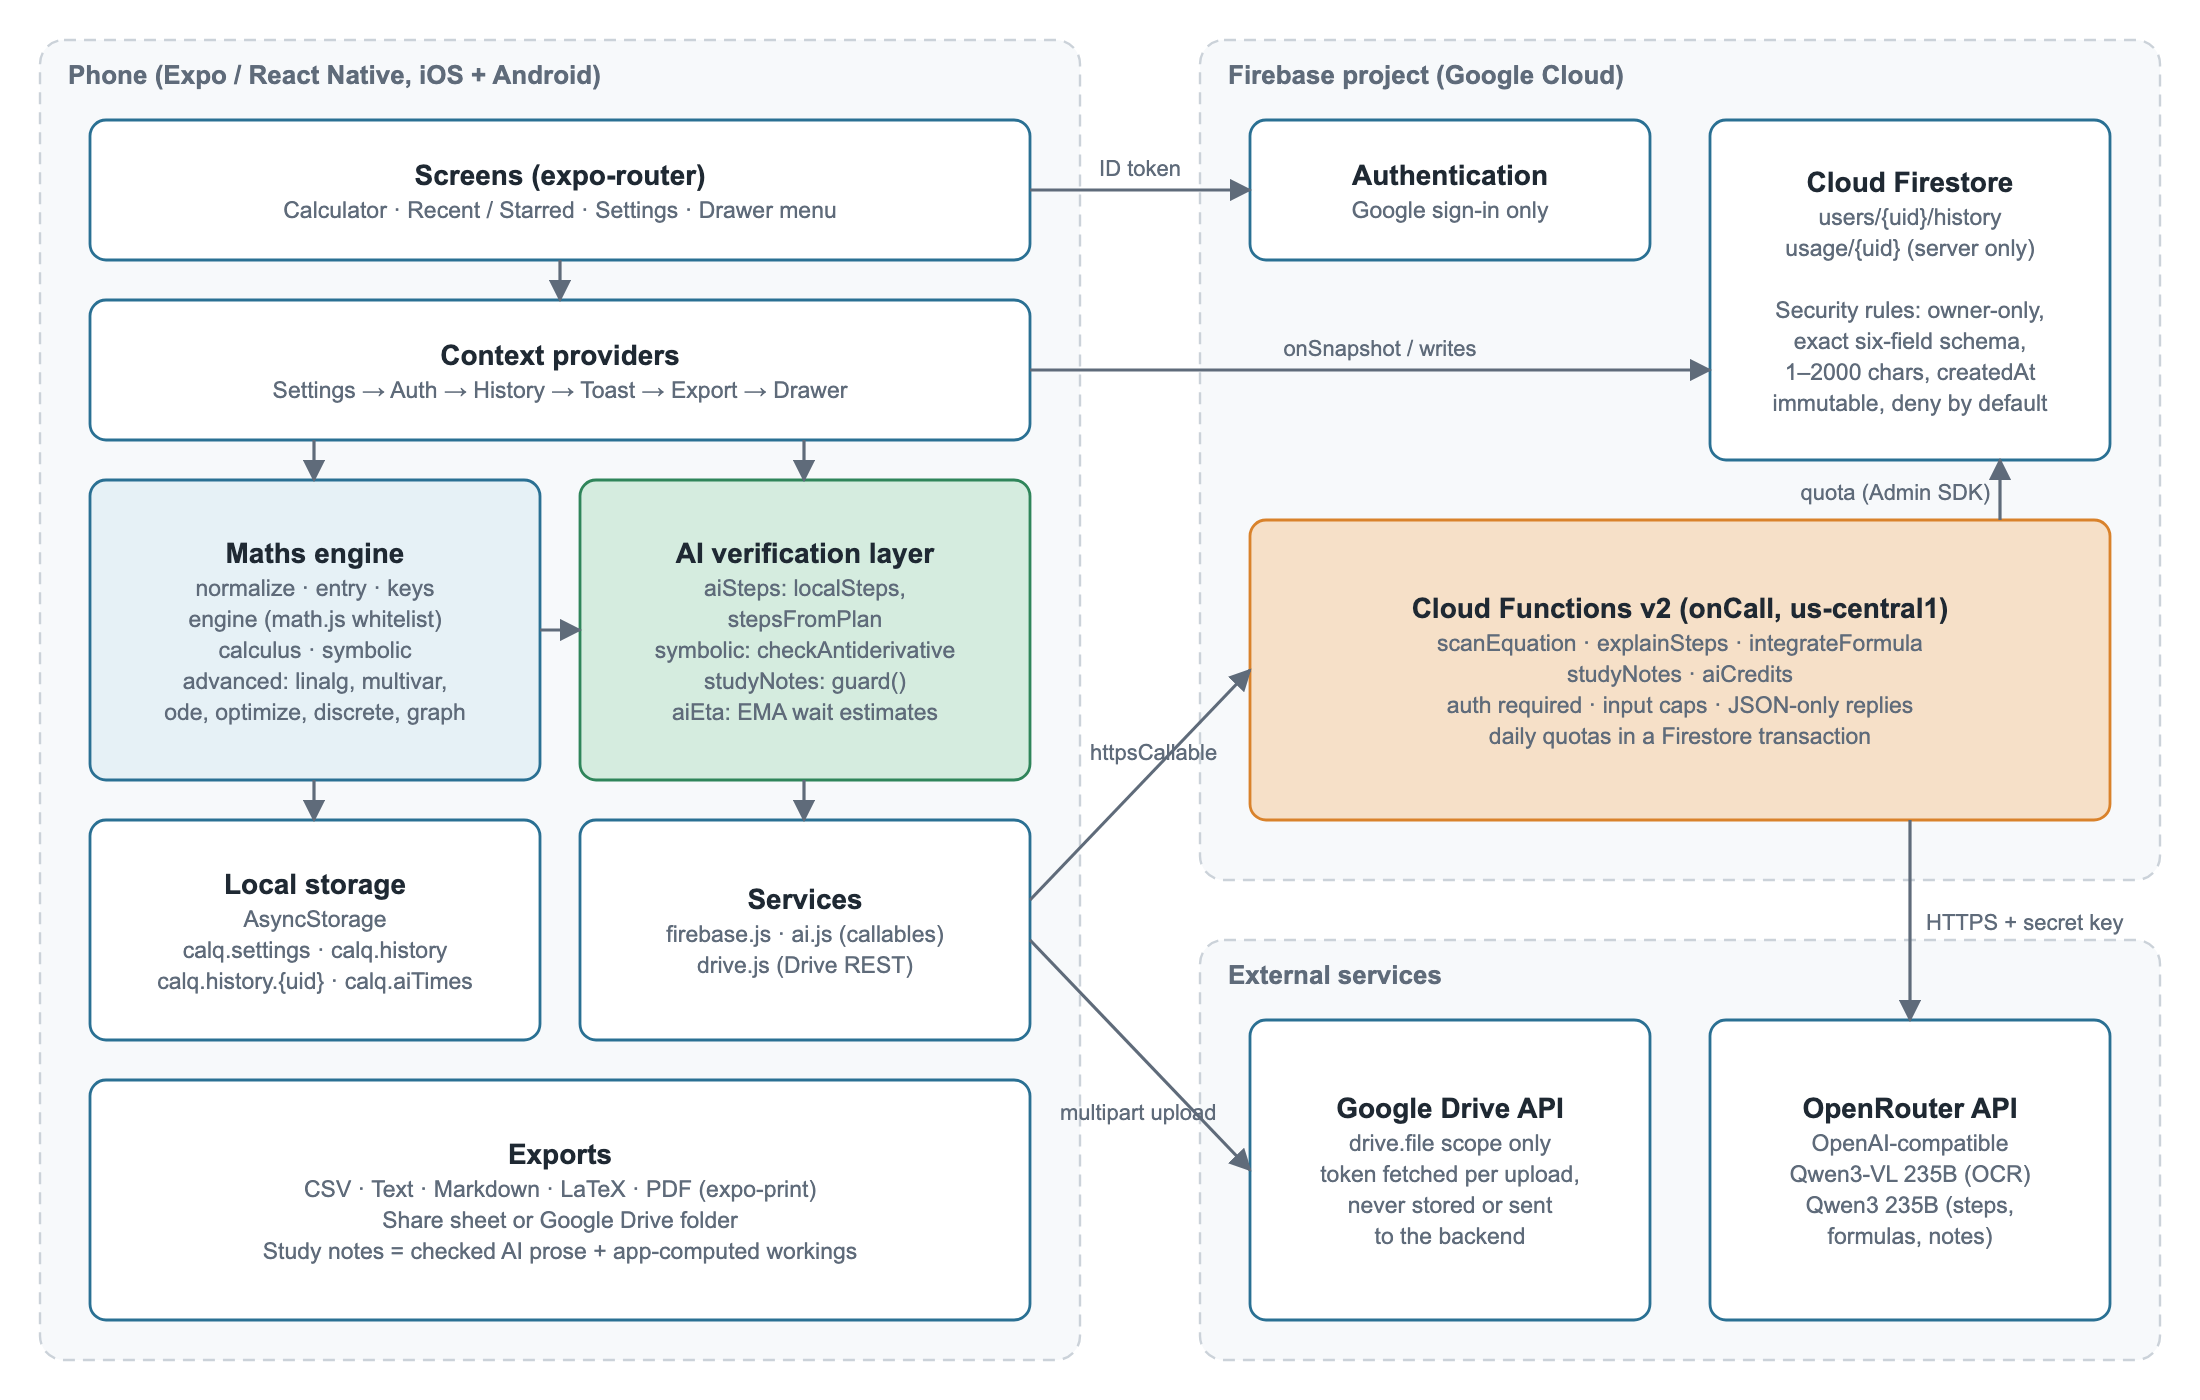
\includegraphics[width=15.5cm]{figures/architecture.png}
\figcaption{Figure 3.1: System architecture: the app (left), the Firebase project (top right) and the external services it calls}{Figure 3.1: System architecture: the app (left), the Firebase project (top right) and the external services it calls}
\end{figblock}

\Htwo{3.1 In scope}{3.1 In scope}

\begin{itemize}
\item \textbf{Calculator app} for iOS and Android: four swipeable keypad pages (NUMERIC, SCIENTIFIC, MATRIX · CALCULUS, SOLVE · DISCRETE), live preview, memory and variables, degree/radian/gradian modes, real or complex numbers, decimal or fraction output, light and dark themes.
\item \textbf{History} that works for guests on the device and syncs for signed-in users, with pin, copy, undo, reopen and multi-select export.
\item \textbf{Exports} in five formats to the share sheet or a Google Drive folder.
\item \textbf{AI help} for signed-in users (scan, step shortcuts, antiderivatives, study notes), each checked on the device and limited by a daily quota.
\item \textbf{Backend}: Google sign-in, Firestore with tested security rules, and five Cloud Functions.
\item \textbf{Quality}: automated tests for the maths, screens, exports and rules; a README that lets a new member build the app from scratch.
\end{itemize}

\Htwo{3.2 Out of scope}{3.2 Out of scope}

\begin{itemize}
\item Graph plotting of functions (on the roadmap; see §8.3).
\item Publishing on the App Store and Google Play. We distributed development builds and an Android APK instead, which needs no paid developer account.
\item Training or fine-tuning our own models. The models are used as provided, only through prompts.
\item Examination use. Calq is a study and revision tool, not a replacement for an SEAB- or NTU-approved calculator.
\end{itemize}

\Htwo{3.3 Changes from the charter}{3.3 Changes from the charter}

The charter planned a calculator with authentication, cloud storage and export. Table 3.1 lists what we added or changed and why. The additions were possible because the frontend and backend took less time than planned once the design was settled (§7.2).

\begin{tableblock}
\begin{tabular}{|>{\raggedright\arraybackslash}p{\dimexpr 0.2600\linewidth - 2\tabcolsep - 1.4\arrayrulewidth\relax}|>{\raggedright\arraybackslash}p{\dimexpr 0.3800\linewidth - 2\tabcolsep - 1.4\arrayrulewidth\relax}|>{\raggedright\arraybackslash}p{\dimexpr 0.3600\linewidth - 2\tabcolsep - 1.4\arrayrulewidth\relax}|}
\hline
\textbf{Change} & \textbf{Reason} & \textbf{Effect on plan} \\ \hline
Added AI scan and step shortcuts & Re-typing long tutorial problems was the slowest part of using a calculator, in our own experience & New Cloud Functions; quota and cost controls needed \\ \hline
Added a verification layer for all AI output & LLM arithmetic errors (§2.2) would undermine trust in a calculator & Became the project’s main technical contribution \\ \hline
Added two advanced keypad pages & EEE modules use matrices, ODEs and optimisation; CAS tools use a different notation & About 2,500 lines of numerical code and 7 test files \\ \hline
Steps computed on the device for everyone & Workings should not depend on sign-in, quota or network & AI is asked only for shortcuts on hard arithmetic \\ \hline
Google Drive export & Students keep notes in Drive; saving there removes a manual step & drive.file scope; consent screen setup \\ \hline
Gradian angle mode & Completeness with handheld calculators & Touched engine, rules and functions; tested end to end \\ \hline
\end{tabular}
\end{tableblock}
\tabcaption{Table 3.1: Scope changes relative to the project charter}{Table 3.1: Scope changes relative to the project charter}

\clearpage
\Hone{4. System Design and Implementation}{4. System Design and Implementation}

This chapter follows a calculation from the key press to the screen, the cloud and the export. The app is 10,434 lines of JavaScript (excluding 3,732 lines of tests), of which 4,702 are the maths engine; the backend is 493 lines of Cloud Functions and a 34-line rules file.

\Htwo{4.1 User interface and experience design}{4.1 User interface and experience design}

\Hthree{4.1.1 Design process}{4.1.1 Design process}

The charter planned to design the interface in Figma. In practice the design members (Chan Wei Kiat, Lee Jie Xuan Gina and Nathaniel Naveen Umaibalan) worked in Claude Design, Anthropic’s AI-assisted design tool, which let them describe a screen, generate a layout and refine it together on a shared canvas. They began in Week 3 by listing what annoyed us about existing calculator apps. By 26 August they had a first home screen for saved calculations, then called CalcMaster, and by 29 August two keypad layouts modelled on a handheld calculator: a numeric layout and a scientific layout (Figure 4.1).

\begin{figblock}
\begin{minipage}[b]{0.604\linewidth}\centering
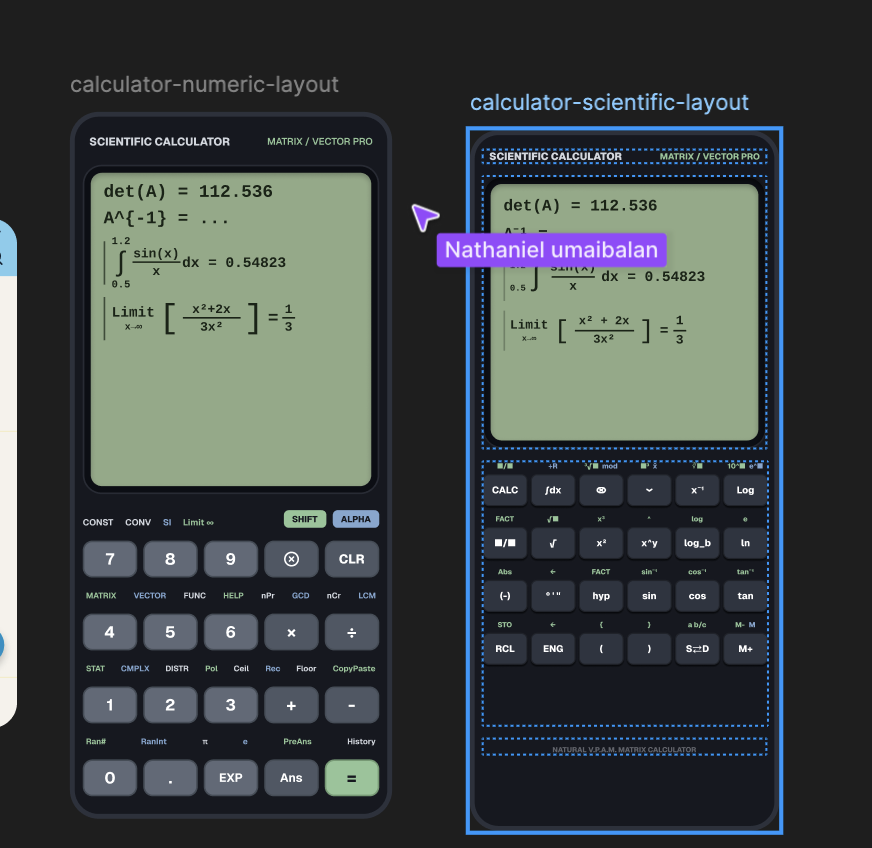
\includegraphics[width=7.4cm]{figures/early_keypads.png}\par\vspace{4pt}
(a) Numeric and scientific keypad layouts, 29 Aug
\end{minipage}\hfill
\begin{minipage}[b]{0.376\linewidth}\centering
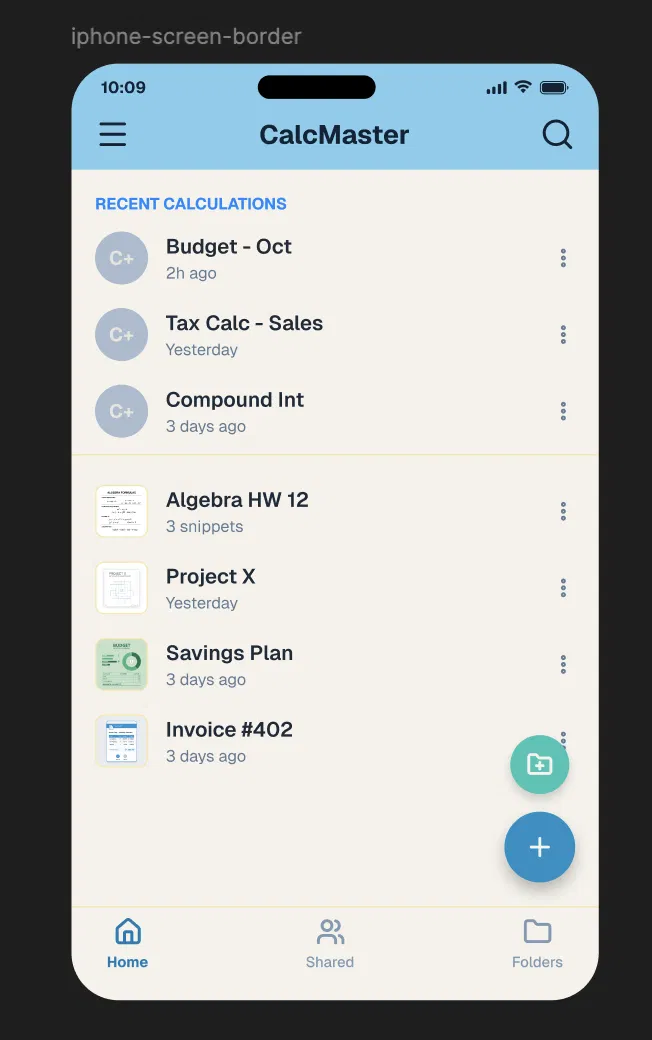
\includegraphics[width=4.6cm]{figures/early_home.png}\par\vspace{4pt}
(b) CalcMaster home screen, 26 Aug
\end{minipage}\par\vspace{6pt}
\figcaption{Figure 4.1: Early layouts in Claude Design (Week 3, before the charter was submitted)}{Figure 4.1: Early layouts in Claude Design (Week 3, before the charter was submitted)}
\end{figblock}

During the recess week the designs were developed in Claude Design into clickable HTML mock-ups, exported from the tool so the whole group could try the layout on a phone-sized frame (Figure 4.2). Two decisions from this stage carried through to the final app: a calm blue palette (header \#A8CFE0, accent \#2A7093) on a warm off-white background, and a keypad split into pages that are swiped rather than one page crowded with tiny keys. Comparing Figure 4.1 with the final app (Figure 4.3) shows the other main change: the green LCD-style display of the early layouts gave way to a scrolling list of past calculations, so that history is always in view.

\begin{figblock}
\begin{minipage}[b]{0.490\linewidth}\centering
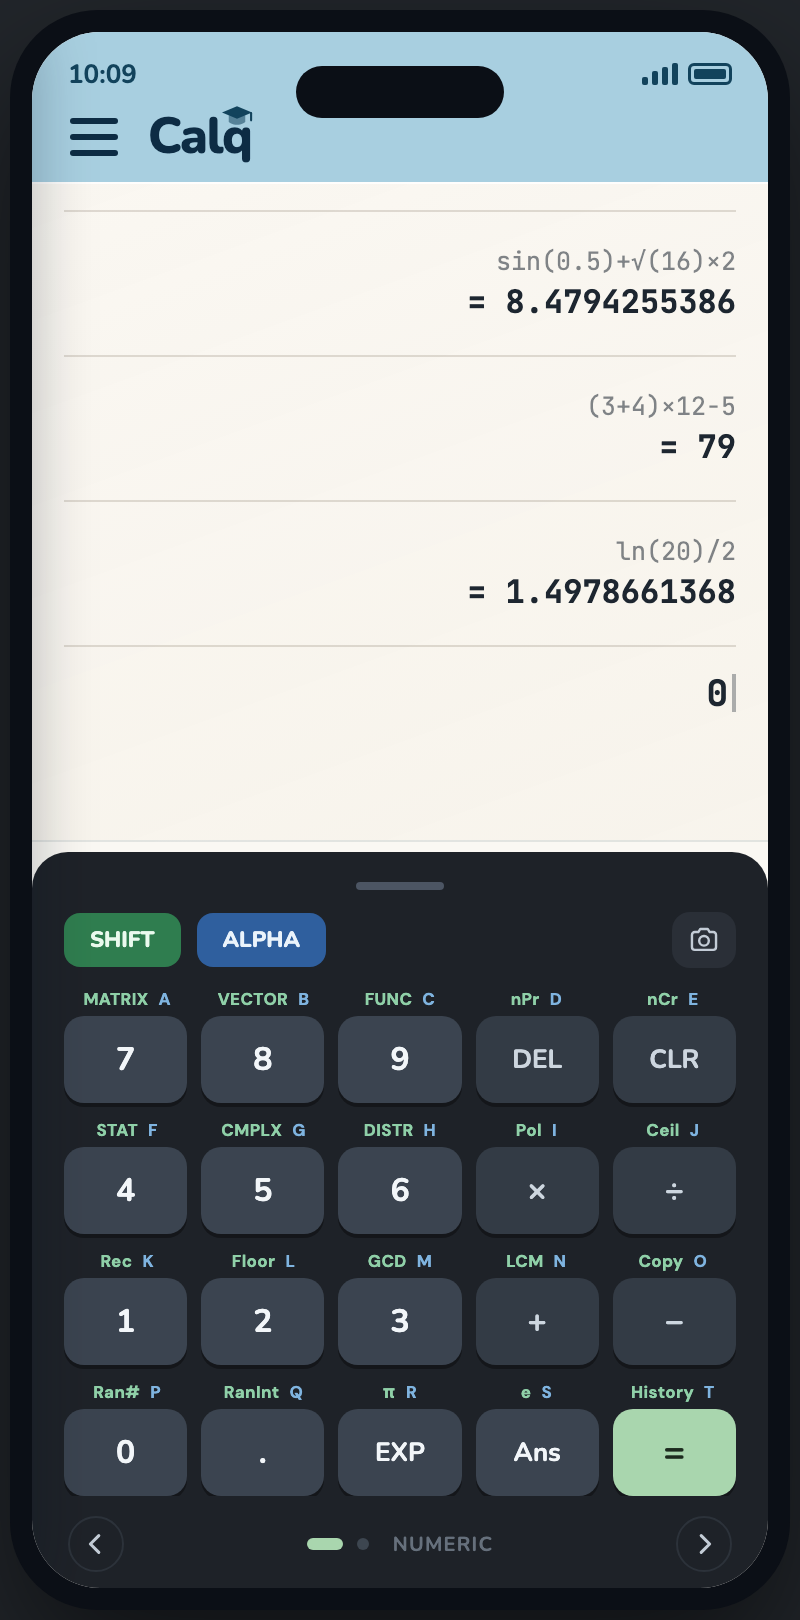
\includegraphics[width=4.3cm]{figures/mock_calc.png}\par\vspace{4pt}
(a) Calculator mock-up
\end{minipage}\hfill
\begin{minipage}[b]{0.490\linewidth}\centering
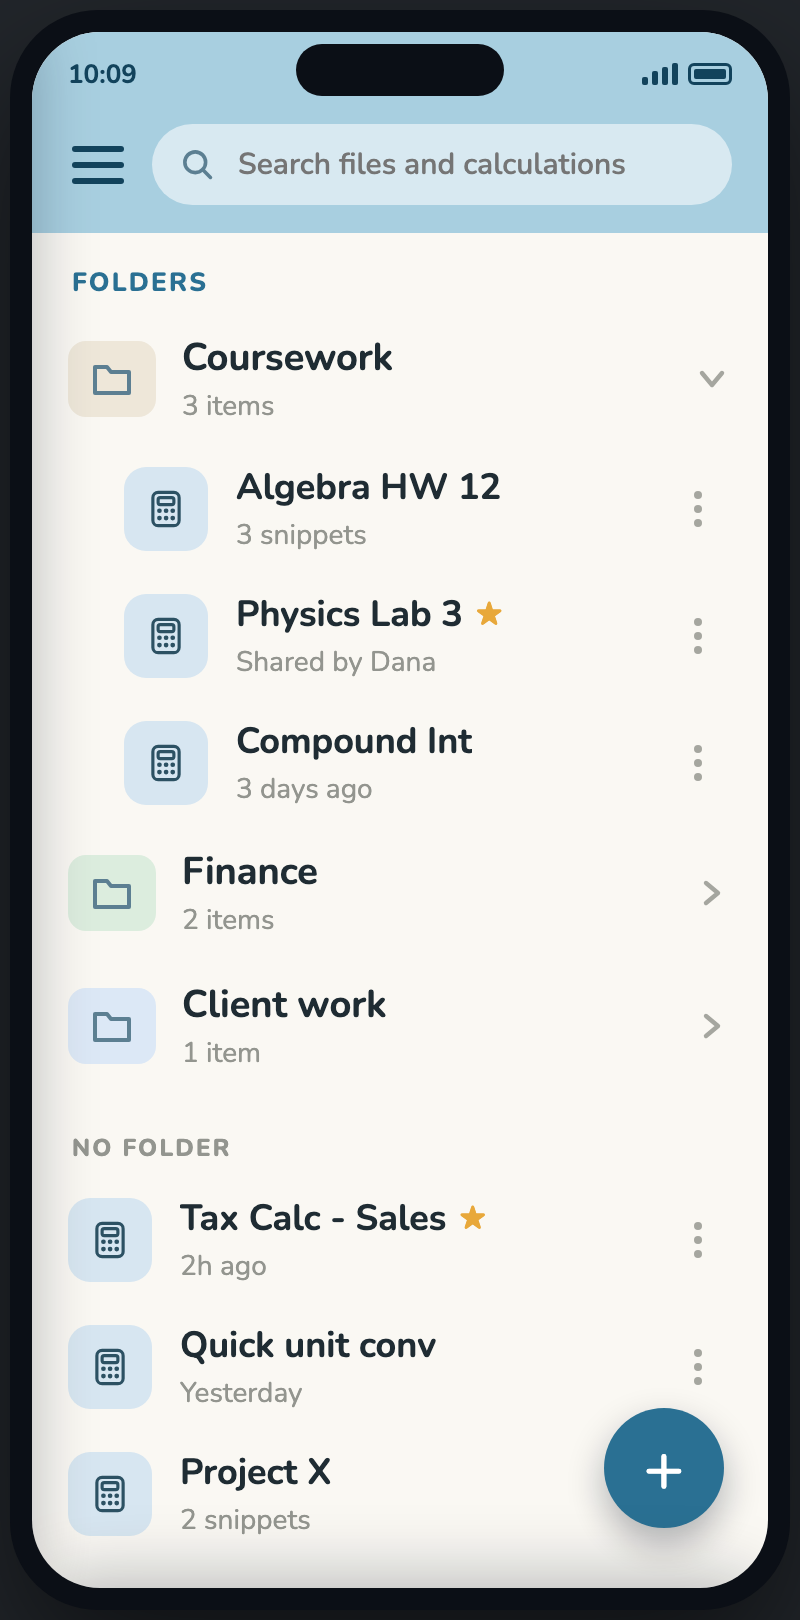
\includegraphics[width=4.3cm]{figures/mock_menu.png}\par\vspace{4pt}
(b) Saved-calculations mock-up
\end{minipage}\par\vspace{6pt}
\figcaption{Figure 4.2: Clickable HTML mock-ups exported from Claude Design during the recess week}{Figure 4.2: Clickable HTML mock-ups exported from Claude Design during the recess week}
\end{figblock}

The mock-up in Figure 4.2(b) organised calculations into folders, like a file manager. Filing every calculation by hand adds work at the moment a student least wants it, and most look-ups are of the last few results. The final app therefore replaced folders with a chronological \textbf{Recent} list and a \textbf{Starred} filter (Figure 4.3(b)), and moved organisation into exports and Google Drive folders. \fillin{[CONFIRM: design team to add the user feedback behind this change, if any]}

\begin{figblock}
\begin{minipage}[b]{0.327\linewidth}\centering
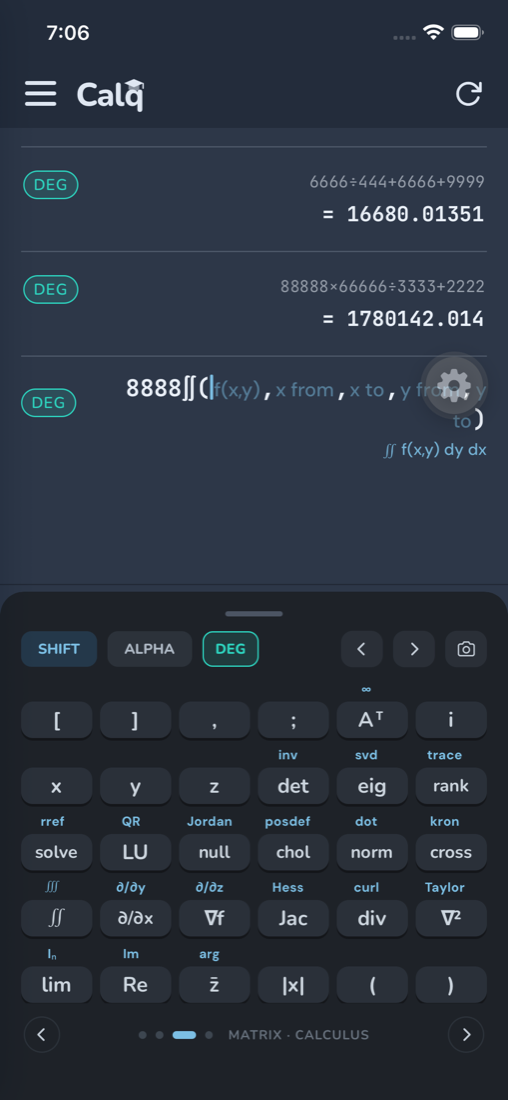
\includegraphics[width=4cm]{figures/shot_calc_matrix.png}\par\vspace{4pt}
(a) Calculator, MATRIX · CALCULUS page
\end{minipage}\hfill
\begin{minipage}[b]{0.327\linewidth}\centering
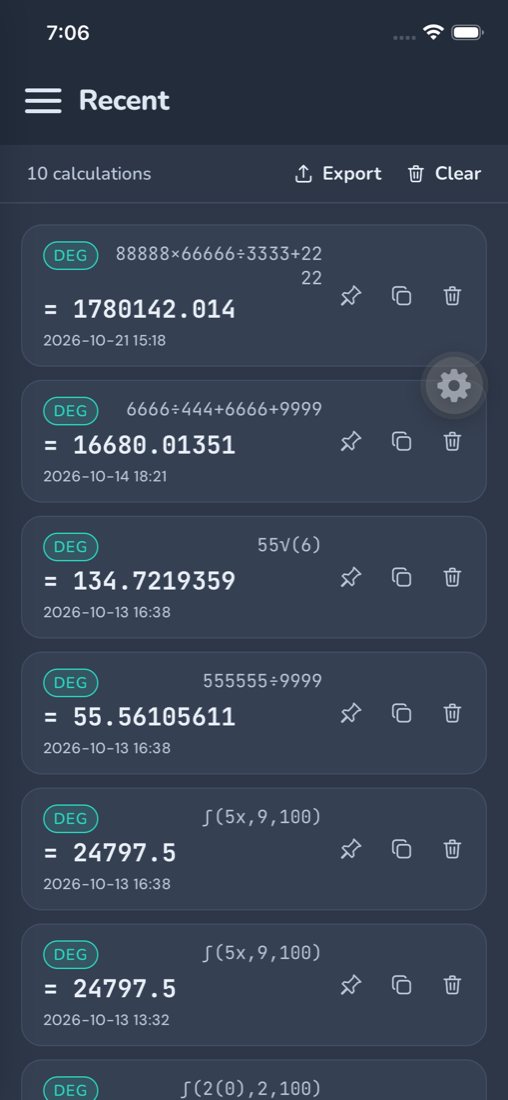
\includegraphics[width=4cm]{figures/shot_history.png}\par\vspace{4pt}
(b) Recent history
\end{minipage}\hfill
\begin{minipage}[b]{0.327\linewidth}\centering
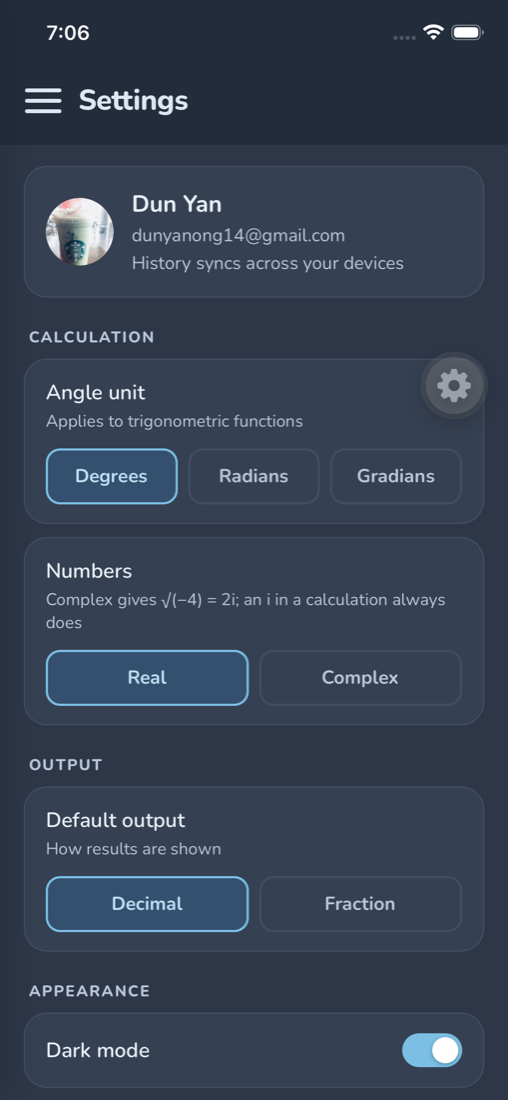
\includegraphics[width=4cm]{figures/shot_settings.png}\par\vspace{4pt}
(c) Settings
\end{minipage}\par\vspace{6pt}
\figcaption{Figure 4.3: The final app on an iPhone 16e (iOS 26.3), dark theme}{Figure 4.3: The final app on an iPhone 16e (iOS 26.3), dark theme}
\end{figblock}

\Hthree{4.1.2 Design principles}{4.1.2 Design principles}

\begin{itemize}
\item \textbf{Familiar first.} The NUMERIC and SCIENTIFIC pages follow the layout of a Casio ClassWiz, with SHIFT and ALPHA labels above each key, so students do not have to relearn where sin\textsuperscript{−1} or nCr live.
\item \textbf{Guided input for many arguments.} Keys such as ∫, ∫∫ or ODE insert a template with labelled boxes, e.g. ∫∫(f(x,y), x from, x to, y from, y to), and a hint line under the entry explains the current box (visible in Figure 4.3(a)). This replaced the error-prone comma counting of handheld calculators.
\item \textbf{Never block the screen.} Slow keys show “Working it out…”, AI waits show a countdown learned from previous calls (§4.5.6), and every destructive action can be undone from a toast.
\item \textbf{One switch for AI.} Settings → AI help hides every AI entry point when off; guests never see AI at all. The disclosure “Your calculations are sent to an AI service to do this” sits next to the switch.
\item \textbf{Accessible type and contrast.} Three type families (Nunito for headings, DM Sans for text, JetBrains Mono for expressions), light and dark palettes defined as tokens, and screen-reader labels on results, matrices, the angle badge and AI progress messages.
\end{itemize}

\Htwo{4.2 Application architecture}{4.2 Application architecture}

The app uses expo-router with four routes: / (calculator), /history (Recent, or Starred with ?filter=pinned) and /settings, plus a slide-in drawer. State lives in React context providers nested in a fixed order, from the outermost: Settings → Auth → History → Toast → Export → Drawer. The order encodes dependencies: history needs to know who is signed in, and exports need both history and toasts. The splash screen stays up until fonts, settings and history have loaded, then fades out over 300 ms, so the user never sees an empty list flash into a full one.

Services are thin modules with no UI: firebase.js initialises Auth (with AsyncStorage persistence), Firestore and Functions; ai.js wraps each Cloud Function with timeouts of 70 s (130 s for notes), user-friendly error messages and a session cache; drive.js talks to the Google Drive REST API. Keeping these separate from the screens let us mock them in tests (§5.2).

\Htwo{4.3 The expression pipeline}{4.3 The expression pipeline}

Figure 4.4 shows the path from a key press to a formatted result. Every calculation, typed or scanned, follows it.

\begin{figblock}
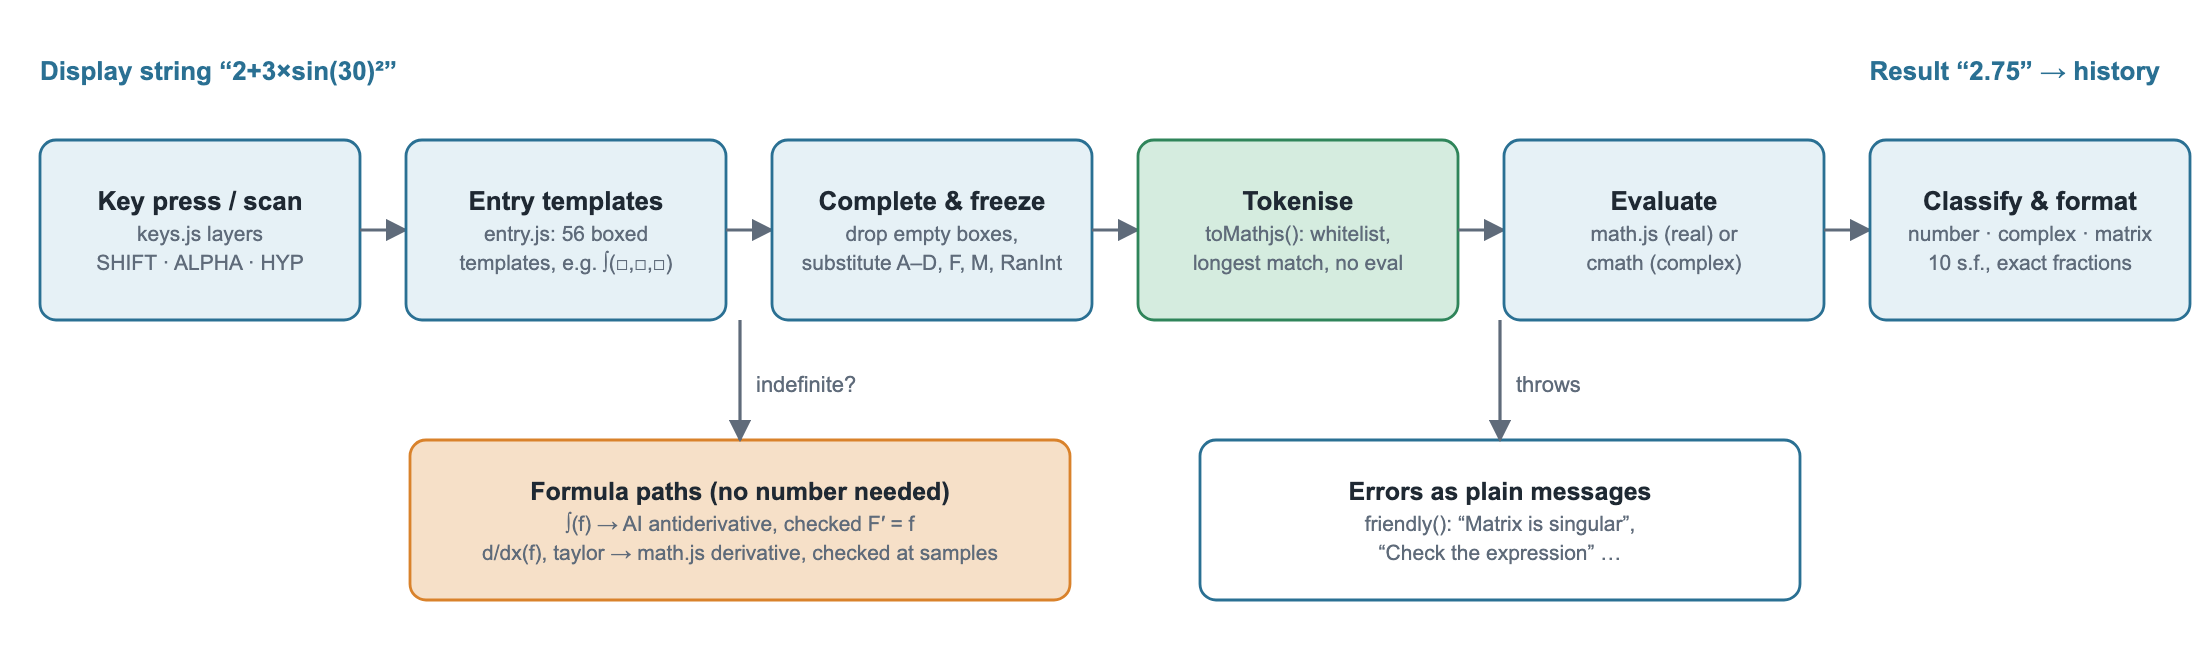
\includegraphics[width=15.9cm]{figures/pipeline.png}
\figcaption{Figure 4.4: From key press to result. The tokeniser (green) is the security boundary: only whitelisted symbols reach math.js}{Figure 4.4: From key press to result. The tokeniser (green) is the security boundary: only whitelisted symbols reach math.js}
\end{figblock}

\Hthree{4.3.1 Keys and templates}{4.3.1 Keys and templates}

keys.js defines the four keypad pages; each key has a main action and optional SHIFT, ALPHA and HYP actions. Keys that need several inputs insert one of 56 templates from entry.js, written with box characters (□) that the cursor jumps between. DEL never breaks a template: DEL on a template’s opening symbol removes the whole template, and a box emptied by DEL shows □ again. When the user presses =, completeEntry drops optional empty boxes, so ∫(f,□,□) becomes ∫(f), an indefinite integral, and d/dx(f,□) becomes a derivative formula.

\Hthree{4.3.2 Tokenising safely}{4.3.2 Tokenising safely}

The display string uses calculator symbols (×, ÷, √, ², sin\textsuperscript{−1}, π) that math.js does not understand. toMathjs() converts it with a longest-match tokenizer over a whitelist of known symbols and function names; anything else is rejected with “Check the expression”. Because the converted string is only ever passed to math.js’s own parser, which has no access to JavaScript, there is no path from user input or a scanned photo to code execution. Implicit multiplication follows the convention students expect: 2π, 3sin(30) and 2(3+4) multiply, and 6÷2(3) evaluates to 9, the same as math.js and most modern calculators.

\Hthree{4.3.3 Angles, numbers and formatting}{4.3.3 Angles, numbers and formatting}

Two math.js instances are created: math with predictable: true, so √(−4) is an error in Real mode, and cmath, which returns complex numbers when Settings → Numbers is Complex or the expression contains i. Trigonometric functions are replaced by wrappers that convert from the current angle unit (360°, 2π rad or 400 grad per turn). tan(90°) is reported as undefined exactly rather than as 1.6×10¹\textsuperscript{6}, and values below 10\textsuperscript{−12} in magnitude are cleaned to 0, so sin(180°) shows 0. format.js prints ten significant figures, switches to scientific notation outside 10\textsuperscript{−7} to 10¹\textsuperscript{0}, and offers a fraction only when it is exact to 10\textsuperscript{−12} with a denominator of at most 10,000.

Results are classified as a number, complex number, matrix, text or a set of named parts (for example x=…, min=…). A number, complex value or matrix goes into Ans, so det(Ans) works after computing a matrix; multi-part results leave Ans unchanged.

\Htwo{4.4 Numerical methods on the device}{4.4 Numerical methods on the device}

All advanced keys run on the phone without AI. advanced.js registers each method as a math.js function; where the first argument is a formula (∫, ∫∫, ode, min), it receives the unevaluated expression and turns it into a JavaScript function of x, y and z. Table 4.1 summarises the methods, and the subsections explain the ones whose design choices matter most.

\begin{tableblock}
\begin{tabular}{|>{\raggedright\arraybackslash}p{\dimexpr 0.1800\linewidth - 2\tabcolsep - 1.4\arrayrulewidth\relax}|>{\raggedright\arraybackslash}p{\dimexpr 0.4000\linewidth - 2\tabcolsep - 1.4\arrayrulewidth\relax}|>{\raggedright\arraybackslash}p{\dimexpr 0.4200\linewidth - 2\tabcolsep - 1.4\arrayrulewidth\relax}|}
\hline
\textbf{Key(s)} & \textbf{Method} & \textbf{Key parameters} \\ \hline
∫ & Adaptive Gauss–Kronrod 7/15 with endpoint-smoothing substitution & tol 10\textsuperscript{−11} relative to ∫|f|; ≤ 20,000 evaluations \\ \hline
d/dx, ∂, grad, Jac, div, curl & Ridders’ extrapolation of central differences; one-sided slope check & h\textsubscript{0} = 10\textsuperscript{−3}·scale; 10 extrapolation rows \\ \hline
Hess, Laplacian & Nested Ridders, symmetrised; Laplacian = trace & — \\ \hline
∫∫, ∫∫∫ & Nested adaptive Gauss–Kronrod & inner tol 10\textsuperscript{−10}; budget 2×10\textsuperscript{6} / 4×10\textsuperscript{6} evaluations \\ \hline
lim & Geometric sequence h = h\textsubscript{0}·2\textsuperscript{−k} with Richardson, then Aitken Δ² & 25 terms; tol 10\textsuperscript{−8}; detects ±∞ \\ \hline
ode, ode2 & Dormand–Prince 5(4), FSAL, adaptive step & rtol 10\textsuperscript{−12}, atol 10\textsuperscript{−14}; ≤ 100,000 steps \\ \hline
bvp & Shooting on the initial slope: secant, then bisection & — \\ \hline
min/max (1-D) & 2,000-point scan, then Brent around the 5 best dips & — \\ \hline
min/max (n-D) & BFGS, 4th-order gradients, Armijo backtracking; Nelder–Mead fallback & gradient tol 10\textsuperscript{−9} \\ \hline
minc/maxc & Augmented Lagrangian with BFGS inner solves & ρ: 10 → 10\textsuperscript{8}; feasibility 10\textsuperscript{−7} \\ \hline
lp, ilp & Two-phase simplex (Bland’s rule); depth-first branch and bound & ε 10\textsuperscript{−9}; ≤ 10,000 nodes \\ \hline
root, nsolve, roots & Brent; damped Newton with secant fallback; Aberth–Ehrlich + Newton polish & — \\ \hline
svd, rank, null, chol, Jordan & One-sided Jacobi SVD; rref with partial pivoting; Cholesky; rank sequence of (A−λI)\textsuperscript{k} & ≤ 60 sweeps; rank tol max(m,n)·ε·σ\textsubscript{1} \\ \hline
prime?, factor, φ, modinv & BigInt Miller–Rabin (13 bases); Pollard’s rho (Brent variant); extended Euclid & exact for n < 3.3×10²\textsuperscript{4} \\ \hline
path, mst, flow, assign, χ(G) & Dijkstra / Bellman–Ford; Kruskal; Edmonds–Karp; Hungarian; backtracking & χ(G) limited to 12 vertices \\ \hline
\end{tabular}
\end{tableblock}
\tabcaption{Table 4.1: Numerical methods implemented in the maths engine}{Table 4.1: Numerical methods implemented in the maths engine}

\Hthree{4.4.1 Definite integrals}{4.4.1 Definite integrals}

A Gauss–Kronrod rule evaluates f at 15 points on an interval and returns two estimates: the 15-point Kronrod value and the 7-point Gauss value that reuses seven of the same points. Their difference is a reliable error estimate at no extra cost. Calq starts with four panels and repeatedly splits the panel with the largest estimated error until the total error falls below 10\textsuperscript{−11} of ∫|f|, or 20,000 evaluations have been used (then it reports that the integral does not converge rather than printing a wrong number).

Integrands such as 1/√x or ln x are infinite at an endpoint, which a closed rule such as Simpson’s cannot evaluate at all. Before integrating, Calq substitutes x = a + (b − a)(3t² − 2t³). The new integrand carries a factor 6t(1 − t) that vanishes at both ends, so the samples cluster near the endpoints and the singularity is softened. Gauss–Kronrod nodes never touch the endpoints, so f is never evaluated there. Chapter 6 shows the effect: errors of 10\textsuperscript{−14} on all three singular test integrals.

\Hthree{4.4.2 Derivatives}{4.4.2 Derivatives}

A single central difference [f(x+h) − f(x−h)]/2h has a truncation error proportional to h² and a rounding error proportional to ε/h, so no step size is good for every function. Ridders’ method computes central differences for a decreasing sequence of h and extrapolates them to h → 0 in a Neville tableau, keeping the entry with the smallest error estimate. Before that, Calq compares the left and right slopes at a step of 10\textsuperscript{−5}; if they differ by more than 5\% it reports that the derivative does not exist (|x| at 0, floor(x) at 1) instead of averaging them into a wrong answer.

\Hthree{4.4.3 Differential equations}{4.4.3 Differential equations}

ode(f, x\textsubscript{0}, y\textsubscript{0}, x\textsubscript{1}) integrates y′ = f(x, y) with the Dormand–Prince 5(4) pair. Each step produces a 5th-order solution and an embedded 4th-order one; their difference estimates the local error, and the next step size is scaled by 0.9·err\textasciicircum{}(−1/5), clamped between 0.2 and 5 times the current step. With tolerances of 10\textsuperscript{−12} relative and 10\textsuperscript{−14} absolute the solver takes small steps only where the solution changes quickly. If the step collapses, as it does when the solution blows up in finite time, the key reports “Solution blows up” instead of a huge number. ode2 rewrites a second-order equation as a first-order system; bvp turns a boundary value problem into a root-finding problem on the unknown initial slope (the shooting method); stab(J) classifies an equilibrium from the trace and determinant of the Jacobian.

\Hthree{4.4.4 Optimisation}{4.4.4 Optimisation}

Unconstrained minimisation in several variables uses BFGS: it builds an approximation of the inverse Hessian from successive gradients, so it converges superlinearly without second derivatives. Gradients use 4th-order central differences, and each step is shortened until it decreases f enough (the Armijo condition). If BFGS stalls, for example on a non-smooth function, the derivative-free Nelder–Mead simplex takes over. Constrained problems such as minc(f, [x+y=1, x≥0], [start]) use an augmented Lagrangian: the constraints enter the objective through multiplier and penalty terms, the penalty weight grows from 10 to at most 10\textsuperscript{8}, and the final multipliers are reported as the KKT λ values, which students can check against a hand derivation. Linear programmes use the two-phase simplex method with Bland’s rule to avoid cycling; integer programmes add depth-first branch and bound.

\Hthree{4.4.5 Exact arithmetic for discrete mathematics}{4.4.5 Exact arithmetic for discrete mathematics}

Number theory keys use JavaScript BigInt so that results such as modpow(3, 200, 13) or the factors of a 20-digit number are exact. Primality uses the Miller–Rabin test with the first 13 primes as bases, which is proven deterministic for n < 3.3×10²\textsuperscript{4}; factorisation uses Pollard’s rho with Brent’s cycle detection. Graph keys take a weight or adjacency matrix, the form used in lectures, and return both the value and the witness, e.g. path([0,1,4;1,0,2;4,2,0],1,3) returns d=3, path=[1,2,3].

\Htwo{4.5 AI features and the verification layer}{4.5 AI features and the verification layer}

Four features use language models. Each follows the loop in Figure 4.5: the app sends a request to a Cloud Function, the model proposes a structured JSON answer, and the phone checks it before anything is shown. If the check fails, the user sees a safe fallback, never the unchecked text.

\begin{figblock}
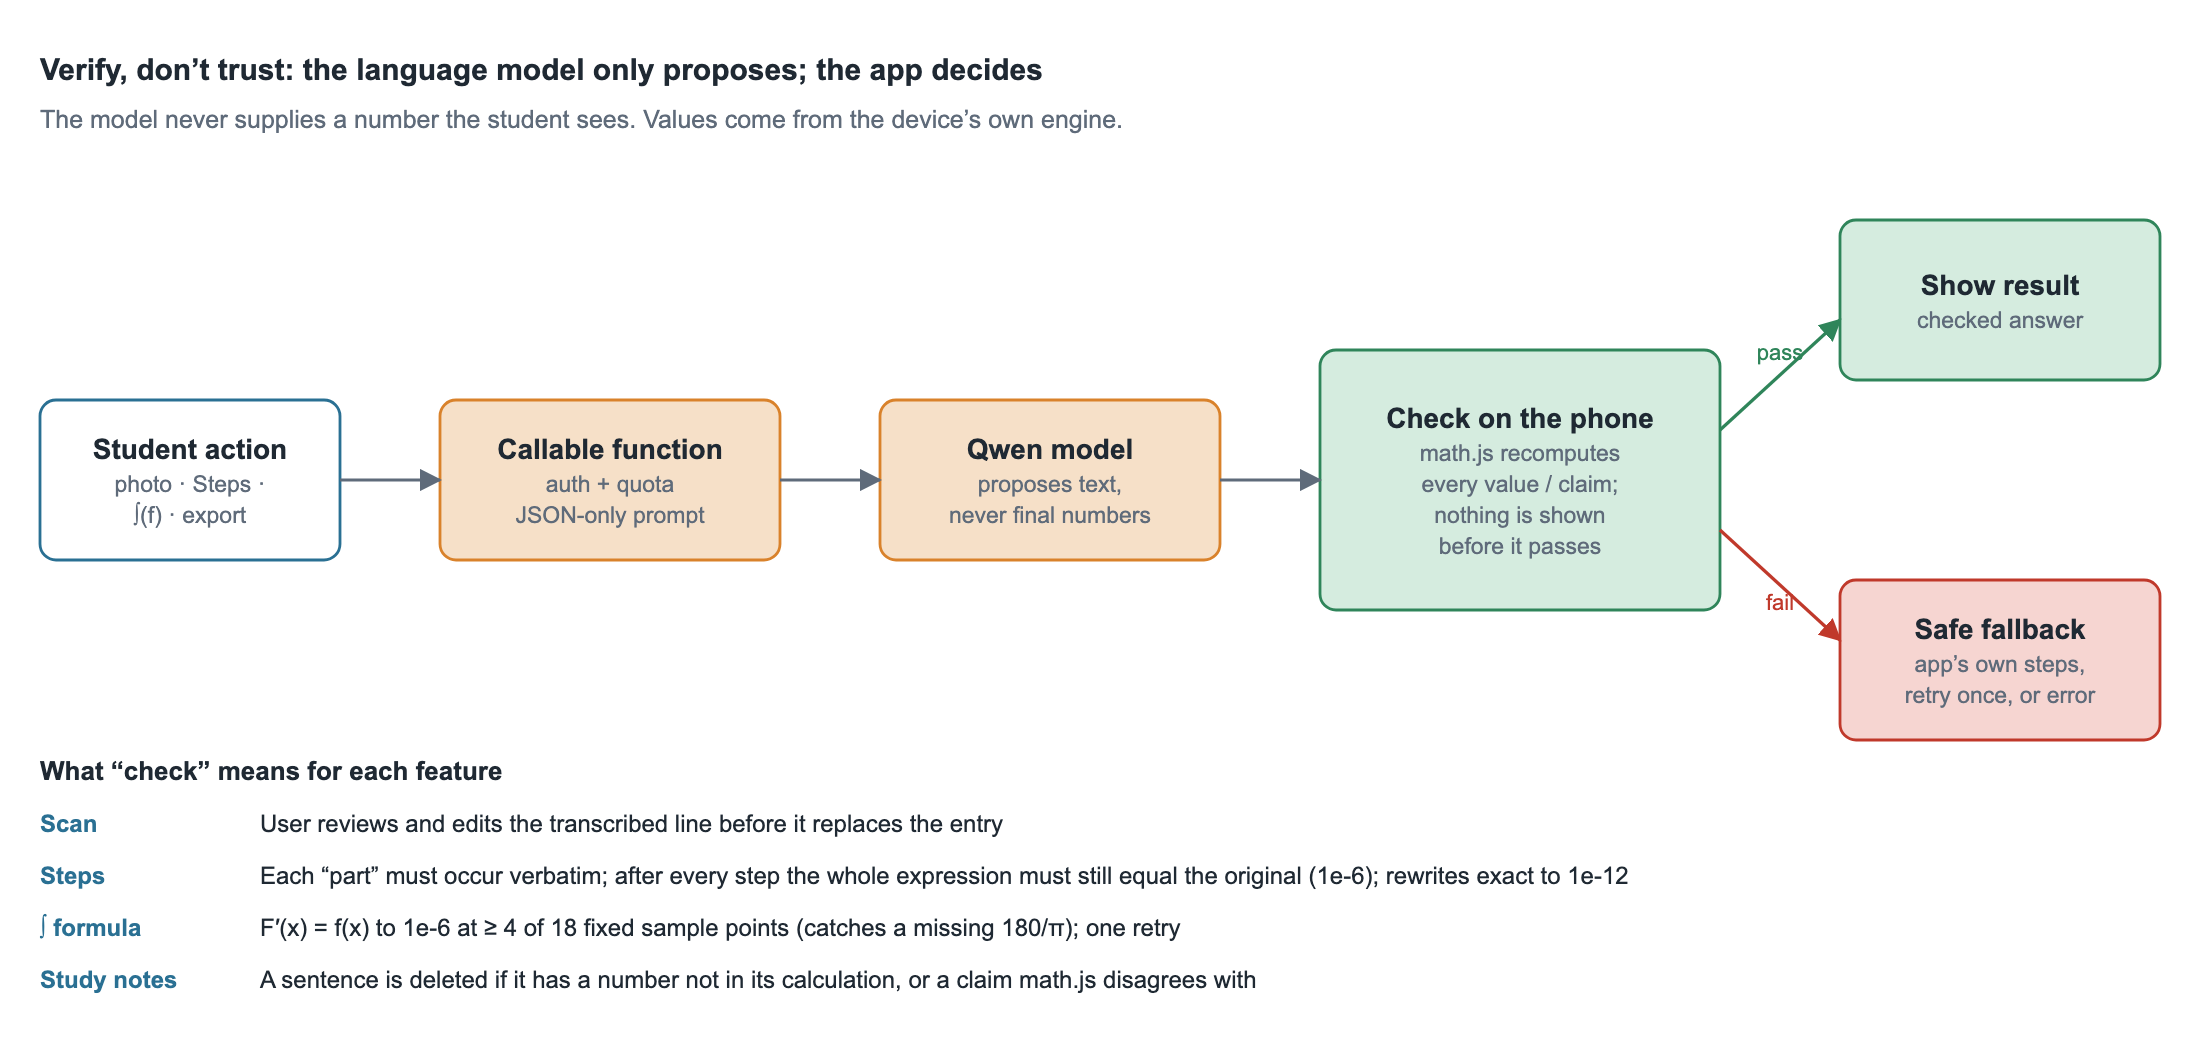
\includegraphics[width=15.9cm]{figures/verify_loop.png}
\figcaption{Figure 4.5: The verify-first loop shared by all AI features, and what “check” means for each}{Figure 4.5: The verify-first loop shared by all AI features, and what “check” means for each}
\end{figblock}

\Hthree{4.5.1 Scan}{4.5.1 Scan}

The camera key on the keypad opens the scan sheet. The photo is resized to at most 1,600 px and compressed to JPEG at quality 0.8 (about 200 KB), then sent to scanEquation, which asks Qwen3-VL to transcribe the problem as one line of Calq notation. The prompt contains about twenty transcription rules, from fractions and matrices to the order of limits in a double integral, and ends with “Do not solve it. Read carefully: 1 vs 7, 5 vs S, 0 vs 6”. The reply is normalised by the same rules as typed input and shown in an editable preview; it replaces the entry only when the user taps Insert. The human review is the check here, because no algorithm can know what was on the paper.

\Hthree{4.5.2 Steps: local first, AI for shortcuts}{4.5.2 Steps: local first, AI for shortcuts}

Holding any calculation with two or more operations and tapping \textbf{Steps} shows its working. In the first version every step came from the AI; we then moved the common case onto the device. localSteps parses the expression with a recursive-descent parser that mirrors math.js precedence (including implicit multiplication), and reduces it in priority order: brackets, functions, powers, multiplication and division, then addition and subtraction, merging chains such as 1+2+3 into one step and labelling each (“Sine of 30°”, “Multiply”). After each reduction the whole expression is evaluated again and must equal the original to a relative 10\textsuperscript{−6}; otherwise no steps are shown. This works instantly, offline and for guests.

The AI is asked only when the arithmetic is hard for a person, such as 489×73. Its plan may contain a \textbf{rewrite} (489×73 → 489×70 + 489×3) and \textbf{parts} to evaluate. stepsFromPlan accepts the plan only if every part occurs verbatim in the current expression without partly overlapping an earlier part, every rewrite equals the original to 10\textsuperscript{−12}, and after each step the whole expression still equals the original to 10\textsuperscript{−6}. The model never supplies a value: the prompt says “Do NOT calculate any numbers. The app computes every value itself”, and the app splices in math.js results. If any check fails the device’s own steps stay on screen.

\begin{figblock}
\begin{minipage}[b]{0.490\linewidth}\centering
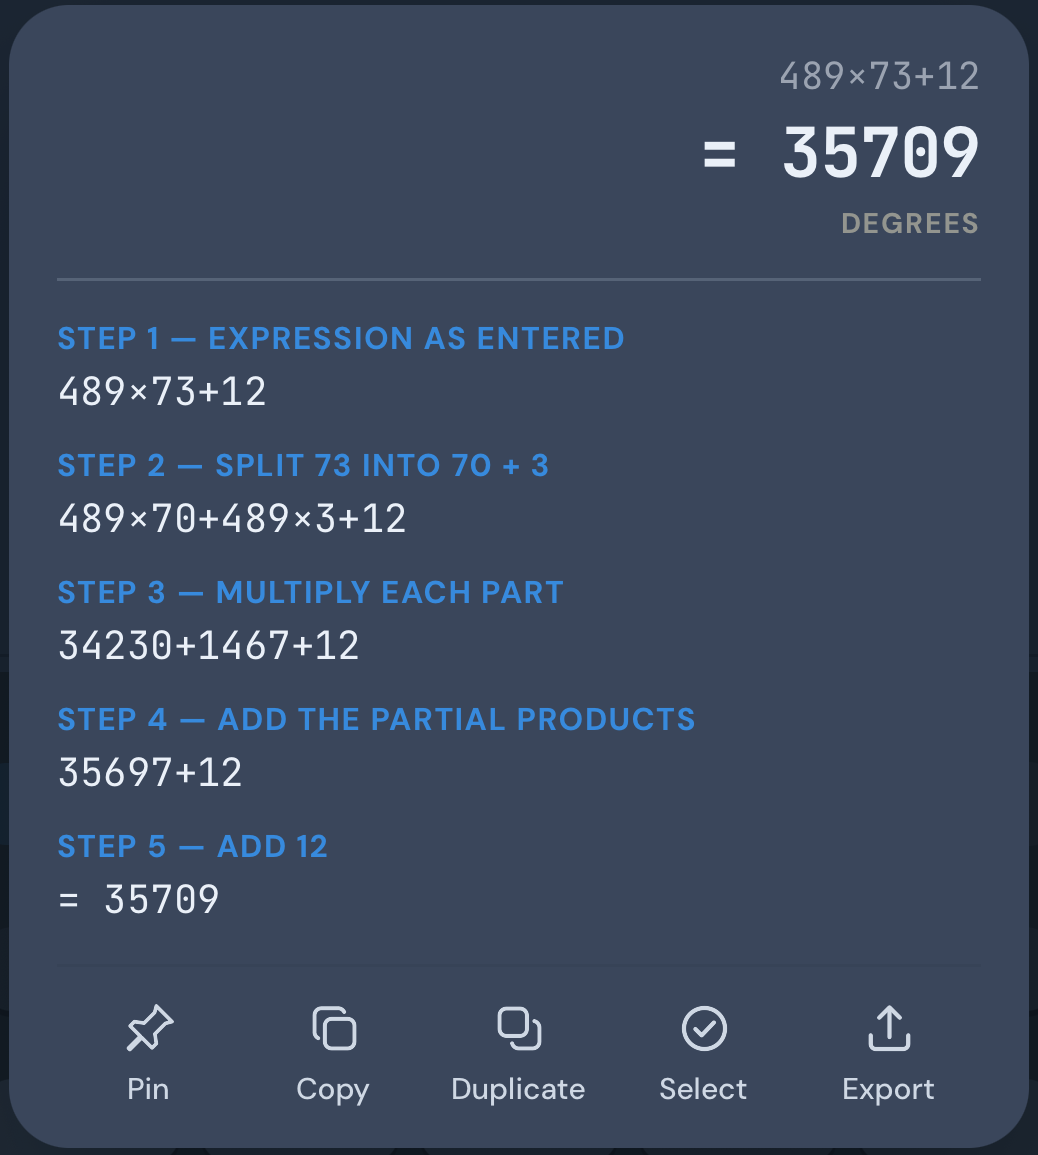
\includegraphics[width=6.2cm]{figures/shot_steps.png}\par\vspace{4pt}
(a) Steps for 489×73+12, with the checked AI shortcut
\end{minipage}\hfill
\begin{minipage}[b]{0.490\linewidth}\centering
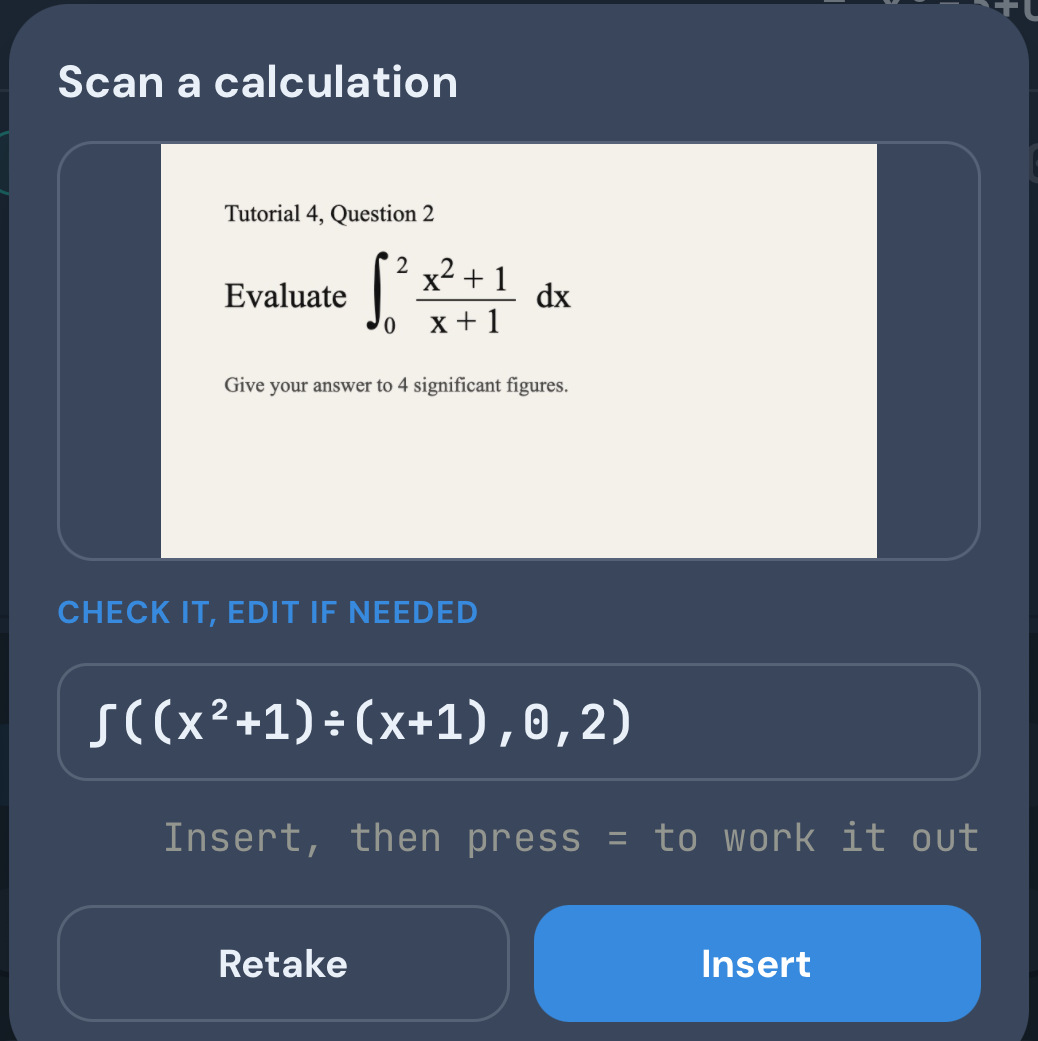
\includegraphics[width=6.2cm]{figures/shot_scan.png}\par\vspace{4pt}
(b) Scan of a printed question, ready to review
\end{minipage}\par\vspace{6pt}

\end{figblock}
\nopagebreak\vspace{8pt}
\begin{figblock}
\begin{minipage}[b]{0.490\linewidth}\centering
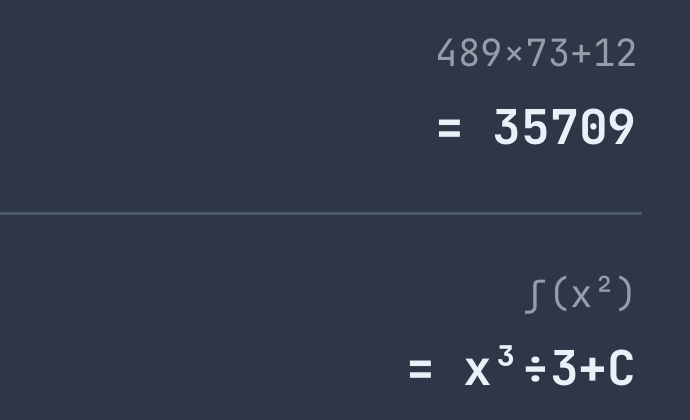
\includegraphics[width=6.2cm]{figures/shot_formula.png}\par\vspace{4pt}
(c) ∫(x²) with empty limits: checked formula
\end{minipage}\hfill
\begin{minipage}[b]{0.490\linewidth}\centering
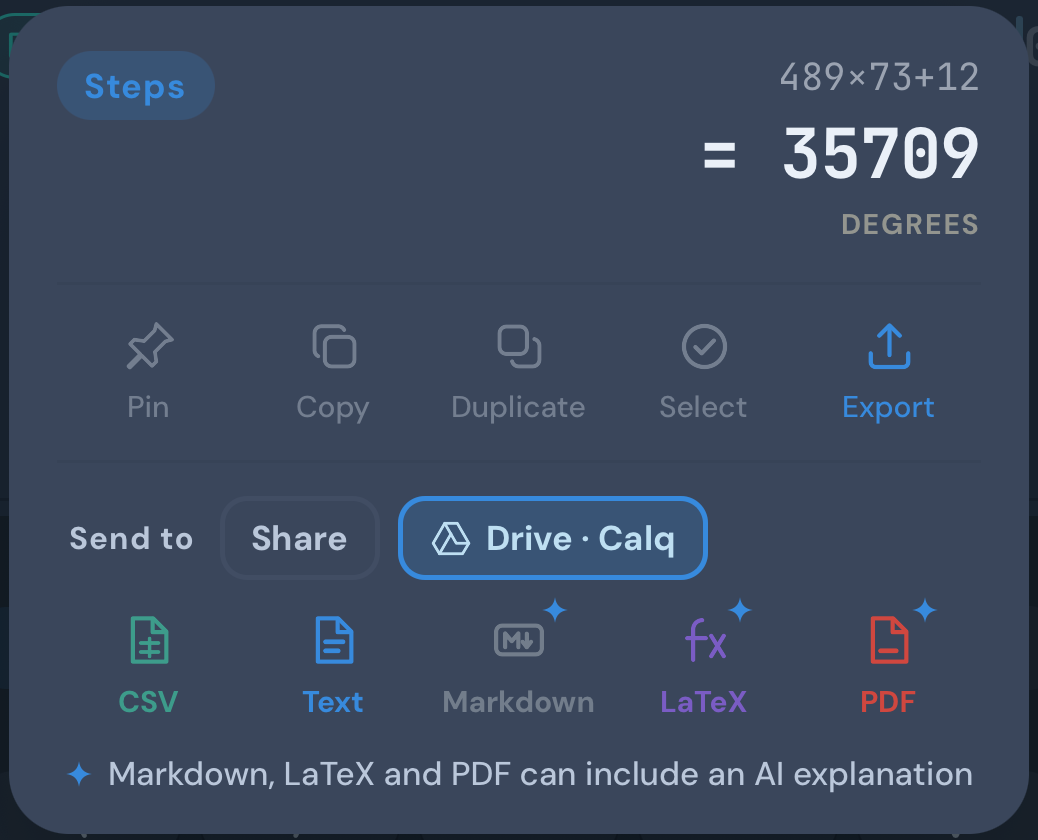
\includegraphics[width=6.2cm]{figures/shot_export.png}\par\vspace{4pt}
(d) Export sheet: five formats, Share or Drive
\end{minipage}\par\vspace{6pt}
\figcaption{Figure 4.6: AI-assisted features and exports in the running app (iPhone 16e simulator)}{Figure 4.6: AI-assisted features and exports in the running app (iPhone 16e simulator)}
\end{figblock}

\Hthree{4.5.3 Antiderivatives}{4.5.3 Antiderivatives}

Typing ∫(x²) with both limits empty asks integrateFormula for an antiderivative F. checkAntiderivative strips any “+C”, differentiates F numerically with Ridders’ method, and accepts it only if F′(x) equals f(x) to a relative 10\textsuperscript{−6} at every one of 18 fixed sample points where both are defined (at least four must be defined). The points (0.13, 0.37, …, −33.3, 47.1) are irregular so that a wrong formula cannot agree with f by coincidence, and spread widely so that a missing factor of 180/π in degree mode, a mistake the prompt specifically warns the model about, is always caught. One retry is made at a higher temperature; if that also fails the user sees “Couldn’t find a formula for this integral”. The prompt also tells the model to return an empty answer for integrands with no elementary antiderivative, such as e\textasciicircum{}(−x²), rather than guess.

\Hthree{4.5.4 Study notes}{4.5.4 Study notes}

When a signed-in user exports Markdown, LaTeX or PDF, Calq asks “Include AI explanation?”. If the answer is yes, the 20 most recent calculations are sent to studyNotes, which splits them into chunks of five and requests, in parallel, an overview and a section per calculation (title, explanation, a reason for each step, a common mistake and a tip). The workings themselves are computed on the device by localSteps, never by the model.

Every piece of returned prose passes through guard(). It removes markup outside backticks, splits the text into sentences, and deletes a sentence if (a) it contains any number that does not appear in that calculation’s expression, result or workings, apart from a small allow-list (0–12, common angles such as 30, 45, 60 and 90, and gradian quarter-turns), or (b) it makes a claim of the form “A is B” or “A = B” that math.js evaluates differently in that calculation’s angle unit. The prompt warns the model about both rules, which in practice makes it write method-focused prose. The app then writes all Markdown, LaTeX and HTML itself, so the model cannot inject formatting.

\Hthree{4.5.5 Prompt design}{4.5.5 Prompt design}

All four prompts share a block that lists Calq’s exact notation, so that model output can be parsed by the app’s own tokenizer. Each prompt demands JSON only with an explicit schema, uses temperature 0 (0.6 on a retry, to get a different answer), and includes one or two worked examples; the full text is in functions/prompts.js. llm.js extracts the first JSON object from the reply even if the model wraps it in a code fence, and maps network failures and malformed replies to clear errors.

\Hthree{4.5.6 Honest waiting times}{4.5.6 Honest waiting times}

An AI call takes several seconds, so each wait shows an estimate (“Reading… \textasciitilde{}8 s left”), then a countdown, then “Taking longer than usual…” if it overruns. aiEta.js learns the estimate per feature on each phone with an exponential moving average, t ← 0.7·t + 0.3·measured, starting from 8 s for scan, 5 s for steps, 6 s for formulas and 15 s for notes, with measurements clamped to 0.5–130 s so a single outlier cannot dominate. Screen readers announce the estimate in words.

\Htwo{4.6 Backend}{4.6 Backend}

\Hthree{4.6.1 Data model and security rules}{4.6.1 Data model and security rules}

\begin{tableblock}
\begin{tabular}{|>{\raggedright\arraybackslash}p{\dimexpr 0.3000\linewidth - 2\tabcolsep - 1.4\arrayrulewidth\relax}|>{\raggedright\arraybackslash}p{\dimexpr 0.4500\linewidth - 2\tabcolsep - 1.4\arrayrulewidth\relax}|>{\raggedright\arraybackslash}p{\dimexpr 0.2500\linewidth - 2\tabcolsep - 1.4\arrayrulewidth\relax}|}
\hline
\textbf{Path} & \textbf{Fields} & \textbf{Written by} \\ \hline
users/\{uid\}/history/\{calcId\} & expr (string, 1–2000), result (string, 1–2000), angle (deg|rad|grad), pinned (bool), createdAt (int), updatedAt (int) & The owner’s app \\ \hline
usage/\{uid\} & day (YYYY-MM-DD), scan, steps, integral, notes (counts) & Cloud Functions only (Admin SDK) \\ \hline
\end{tabular}
\end{tableblock}
\tabcaption{Table 4.2: Firestore data model}{Table 4.2: Firestore data model}

firestore.rules allows a user to read, create, update and delete only documents under their own users/\{uid\} path. A created or updated item must have exactly the six fields above, with the stated types and lengths, and an update may not change createdAt. The calculation id is a client-generated UUID of at most 64 characters, which makes writes idempotent (§4.7). Everything else, including usage/, is denied to clients by default. The 2,000-character limit was raised from 200 when the advanced keys arrived, because an SVD result or a 4×4 matrix exceeds 200 characters.

\Hthree{4.6.2 Cloud Functions}{4.6.2 Cloud Functions}

\begin{tableblock}
\begin{tabular}{|>{\raggedright\arraybackslash}p{\dimexpr 0.2000\linewidth - 2\tabcolsep - 1.4\arrayrulewidth\relax}|>{\raggedright\arraybackslash}p{\dimexpr 0.3200\linewidth - 2\tabcolsep - 1.4\arrayrulewidth\relax}|>{\raggedright\arraybackslash}p{\dimexpr 0.4800\linewidth - 2\tabcolsep - 1.4\arrayrulewidth\relax}|}
\hline
\textbf{Function} & \textbf{Model and limits} & \textbf{Returns} \\ \hline
scanEquation & Qwen3-VL-235B; image ≤ 3 MB base64; 600 tokens & \{ expr ≤ 2000 chars, note ≤ 80 \} \\ \hline
explainSteps & Qwen3-235B; expr ≤ 2000; 1,200 tokens & ≤ 12 steps, ≤ 8 parts each \\ \hline
integrateFormula & Qwen3-235B; 400 tokens & \{ F \} (empty if no elementary form) \\ \hline
studyNotes & Qwen3-235B; 1–20 items in chunks of 5, run in parallel; 120 s timeout & Overview + one section per calculation \\ \hline
aiCredits & No model; uses no quota & \{ used, limit \} across all four quotas \\ \hline
\end{tabular}
\end{tableblock}
\tabcaption{Table 4.3: Cloud Functions (all v2 onCall, sign-in required)}{Table 4.3: Cloud Functions (all v2 onCall, sign-in required)}

Each function validates its input (type, length, base64 pattern), truncates its output, and charges the caller’s daily quota inside a Firestore transaction so that two simultaneous requests cannot both pass the limit. The defaults are 30 scans, 200 step requests, 50 formulas and 20 study-note exports per user per day, reset at 00:00 UTC; the menu shows the share left as “AI credits · N\% left today”. The API key is stored as a Cloud Functions secret and never reaches the phone. The provider URL and both model names are deployment parameters, so the team can switch provider or model without a code change.

\Htwo{4.7 History, sync and offline behaviour}{4.7 History, sync and offline behaviour}

\begin{figblock}
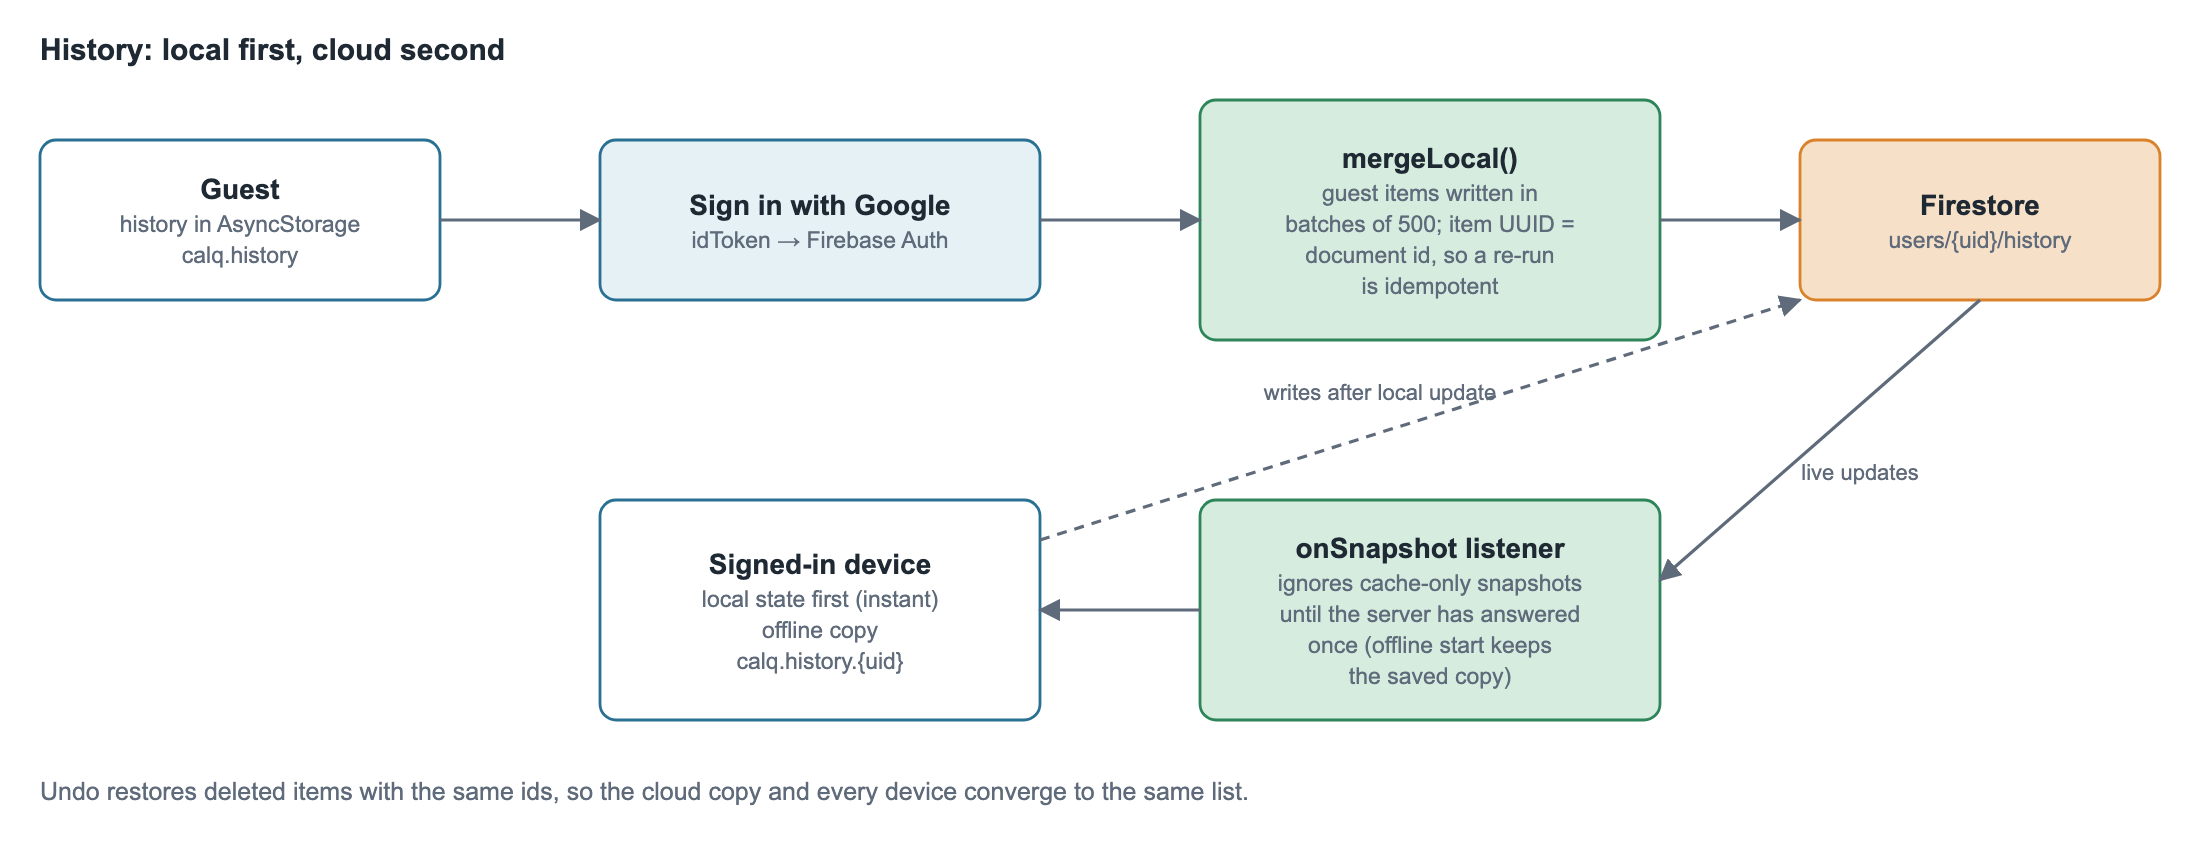
\includegraphics[width=15.5cm]{figures/sync.png}
\figcaption{Figure 4.7: History is local first; signed-in users sync through Firestore and merge guest history on sign-in}{Figure 4.7: History is local first; signed-in users sync through Firestore and merge guest history on sign-in}
\end{figblock}

Every change to history updates the screen first and is then written to the device (AsyncStorage) and, if signed in, to Firestore. On sign-in, the guest history is merged into the cloud in batches of 500 writes. Because each item’s UUID is also its document id, an interrupted merge can simply be repeated without creating duplicates, which our rules tests confirm (§6.1). A real-time onSnapshot listener keeps every device up to date.

One subtle bug shaped this design. When the app started offline, Firestore’s listener immediately delivered an empty snapshot from its local cache, and the app replaced the saved history with nothing. The fix was to ignore cache-only snapshots until the server has answered once; until then the device’s own copy (calq.history.\{uid\}) is shown. Undo restores deleted items with their original ids, so a delete followed by Undo converges on every device.

\Htwo{4.8 Exports and Google Drive}{4.8 Exports and Google Drive}

Exports can come from one calculation (hold → Export), a selection (hold → Select, tap others, then Export) or the whole history. CSV and text contain the calculations only; Markdown, LaTeX and PDF optionally include the checked study notes followed by a plain table of every calculation. PDF is produced on the device from HTML with expo-print.

The \textbf{Send to} switch (Figure 4.6(d)) chooses between the system share sheet and Google Drive. Drive access uses only the drive.file scope, which lets Calq see and change only files and folders it created. Calq requests the scope through the existing Google sign-in only when the user taps Connect, checks that the chosen Google account matches the signed-in Calq account, and fetches a fresh access token for each upload. Tokens are never stored and never sent to our backend; settings keep only the folder name and id. Disconnect revokes Calq’s Google access but leaves the user signed in.

\Htwo{4.9 Security and privacy summary}{4.9 Security and privacy summary}

\begin{tableblock}
\begin{tabular}{|>{\raggedright\arraybackslash}p{\dimexpr 0.3000\linewidth - 2\tabcolsep - 1.4\arrayrulewidth\relax}|>{\raggedright\arraybackslash}p{\dimexpr 0.7000\linewidth - 2\tabcolsep - 1.4\arrayrulewidth\relax}|}
\hline
\textbf{Threat} & \textbf{Mitigation} \\ \hline
Reading or changing another user’s history & Owner-only security rules; 16 emulator tests (§6.1) \\ \hline
Malformed or oversized documents & Exact six-field schema, type and length checks in rules \\ \hline
Code injection through typed or scanned text & Whitelist tokenizer; math.js parser has no access to JavaScript \\ \hline
AI provider key theft & Key held as a Cloud Functions secret; the app calls only authenticated functions \\ \hline
Cost abuse of AI features & Per-user daily quotas in a transaction; input size caps \\ \hline
Over-broad Google access & drive.file scope only, requested on demand; tokens not stored \\ \hline
Wrong answers presented as fact & Verification layer: no unchecked AI number is ever shown \\ \hline
Sending data to AI without consent & AI off for guests; one visible switch with a disclosure sentence \\ \hline
\end{tabular}
\end{tableblock}
\tabcaption{Table 4.4: Threats considered and how Calq addresses them}{Table 4.4: Threats considered and how Calq addresses them}

\Htwo{4.10 Worked example: one calculation end to end}{4.10 Worked example: one calculation end to end}

To tie the chapter together, we follow one calculation, 2+3×sin(30)² in degree mode, through every layer. The outputs below are the app’s real outputs, captured from its modules.

\begin{enumerate}
\item \textbf{Input.} The user presses 2, +, 3, ×, sin, 30, ), x². The entry shows 2+3×sin(30)²; the live preview already reads 2.75.
\item \textbf{Tokenise.} toMathjs produces 2+3*tsin(30)\textasciicircum{}2, where tsin is Calq’s angle-aware sine. Every symbol was on the whitelist.
\item \textbf{Evaluate and format.} math.js returns the number 2.75; classify marks it as a number, format.js prints 2.75, and it becomes Ans.
\item \textbf{Save.} The history context adds the item to the screen, writes it to AsyncStorage and, for a signed-in user, to Firestore, where the rules accept it because it has exactly the six allowed fields.
\item \textbf{Steps.} Holding the item and tapping Steps runs localSteps, which needs no AI, and shows five lines (2+3×0.5², 2+3×0.25, 2+0.75, = 2.75 after the expression itself), each re-evaluated to 2.75.
\item \textbf{Export.} In a LaTeX export the expression is converted by toLatexMath; with AI notes on, studyNotes adds prose about the order of operations, and guard() keeps only sentences whose numbers appear in those lines.
\end{enumerate}

The history item stored in Firestore at users/\{uid\}/history/\{uuid\}:

\codeblock{\{ "expr": "2+3×sin(30)²", "result": "2.75", "angle": "deg",\\
\hspace*{1em}"pinned": false, "createdAt": <ms>, "updatedAt": <ms> \}}

{\raggedright In a LaTeX export, toLatexMath writes the calculation as 2+3\textbackslash{}times \textbackslash{}sin\textbackslash{}left(30\textbackslash{}right)\textasciicircum{}\{2\} = 2.75.\par}

\clearpage
\Hone{5. Testing Methodology}{5. Testing Methodology}

Calq is tested at four levels, from fast unit tests that run on every change to hands-on checks on phones, and every objective in Table 1.1 has evidence behind it.

\Htwo{5.1 Automated tests}{5.1 Automated tests}

\begin{itemize}
\item \textbf{Unit tests} (Jest) for every maths module, the verifiers, exports and settings validation. Each numerical method is tested against closed-form answers, edge cases (singularities, blow-up, singular matrices) and its error messages.
\item \textbf{Component tests} (React Native Testing Library) render the calculator, hold panel, history, scan sheet, exports and settings with Firebase, AI and Drive mocked in jest.setup.js, then press keys and check what the user would see.
\item \textbf{Security rule tests} run firestore.rules against the local Firestore emulator using @firebase/rules-unit-testing, signed in as the owner, as another user and as a guest.
\item \textbf{Static analysis}: ESLint with the Expo configuration over the app, Cloud Functions and tests.
\end{itemize}

In total there are 29 test files: 28 Jest suites with 530 tests, and one rules suite with 16 tests. 

\Htwo{5.2 Benchmarks against baselines}{5.2 Benchmarks against baselines}

To show that Calq’s numerical methods are worth it, we benchmarked the app’s real modules against the simpler methods most calculators and student codes use:

\begin{itemize}
\item \textbf{Integration}: adaptive Gauss–Kronrod against composite Simpson’s rule with 100 intervals (101 evaluations) and the trapezoidal rule with 1,000 intervals, on 12 integrals with known values, three of them singular at an endpoint and one with a square-root kink.
\item \textbf{Differentiation}: Ridders’ method against a single central difference with h = 10\textsuperscript{−3}, 10\textsuperscript{−5} and 10\textsuperscript{−8} at eight points chosen to include steep and near-singular cases.
\item \textbf{ODEs}: Dormand–Prince against classical RK4 with h = 0.01 and Euler with h = 0.001 on five problems with exact solutions, including a stiff-ish one (y′ = −50(y − cos x)) and one that blows up shortly after the end point (y′ = y²).
\item \textbf{Reference values}: 40 calculations across every key family, from 2+3×4 to Bell numbers, each compared with an exact or high-precision value.
\end{itemize}

\Htwo{5.3 Fault injection for the AI verifiers}{5.3 Fault injection for the AI verifiers}

To prove the checkers work, we fed them correct AI answers alongside answers corrupted in exactly the ways language models fail, and measured what each one let through:

\begin{tableblock}
\begin{tabular}{|>{\raggedright\arraybackslash}p{\dimexpr 0.2500\linewidth - 2\tabcolsep - 1.4\arrayrulewidth\relax}|>{\raggedright\arraybackslash}p{\dimexpr 0.4500\linewidth - 2\tabcolsep - 1.4\arrayrulewidth\relax}|>{\raggedright\arraybackslash}p{\dimexpr 0.3000\linewidth - 2\tabcolsep - 1.4\arrayrulewidth\relax}|}
\hline
\textbf{Checker} & \textbf{Corruptions injected} & \textbf{Correct cases / corrupted} \\ \hline
Antiderivative (F′ = f) & Wrong constant factor (×2, ÷2, missing 180/π or 200/π), sign error, wrong power, extra or missing term, wrong function & 15 / 33 \\ \hline
Step plan & Rewrite off by one or with a dropped term, part not in the expression, precedence error, partial overlap & 8 / 17 \\ \hline
Study-notes guard & False value claims, invented numbers, claim true only in another angle unit & 11 / 14 \\ \hline
\end{tabular}
\end{tableblock}
\tabcaption{Table 5.1: Fault types injected}{Table 5.1: Fault types injected}

The comparison is what other AI maths tools do: show the model’s output directly, catching none of these mistakes. Every rejection by Calq is an error that would otherwise have reached a student.

\Htwo{5.4 Manual testing on devices}{5.4 Manual testing on devices}

Each feature was tried on the iOS Simulator (iPhone 16e, iOS 26.3) and the Android emulator (Pixel, Google Play image) before merging, and on members’ own phones through development builds and the release APK \fillin{[FILL IN: list the physical phones and OS versions used]}. Manual checks covered what automated tests cannot: Google sign-in on both platforms, real Firestore sync between two devices, the camera and photo library, PDF rendering, Drive uploads, dark mode and small-screen layout.

\clearpage
\Hone{6. Results and Evaluation}{6. Results and Evaluation}

\Htwo{6.1 Automated test results}{6.1 Automated test results}

All 546 automated tests pass: 530 Jest tests in 28 suites and 16 security-rule tests against the emulator. ESLint reports no errors. Jest measures 92.1\% line coverage across the app, and 96.3\% on the maths engine that every result depends on.

The security rules are proven by tests: an owner can create, read, list, update and delete their own items; that writing the same item twice succeeds (so the sign-in merge is idempotent); that another user or a signed-out client can do none of these; that paths outside users/\{uid\}/history are denied; and that extra or missing fields, empty or over-long strings, unknown angle units, non-boolean pinned, non-integer timestamps and changes to createdAt are all rejected.

\Htwo{6.2 Accuracy on reference values}{6.2 Accuracy on reference values}

All 40 reference calculations matched their exact values to a relative error of 10\textsuperscript{−8}; the largest error was 1.2×10\textsuperscript{−12}. The set spans arithmetic and precedence (6÷2(3) = 9), trigonometry in all three angle units, e\textasciicircum{}(iπ)+1 = 0, definite and singular integrals, derivatives in degree mode (d/dx sin x at 0 = π/180), Σ over 100,000 terms, determinants and ranks, ∫∫ and ∫∫∫, ODEs, Brent root finding, Euler’s totient, modular powers, and Catalan and Bell numbers. Calq was so reliable that, while building this set, it caught an error in one of our own hand-computed determinants.

\Htwo{6.3 Integration against Simpson and trapezoid}{6.3 Integration against Simpson and trapezoid}

\begin{figblock}
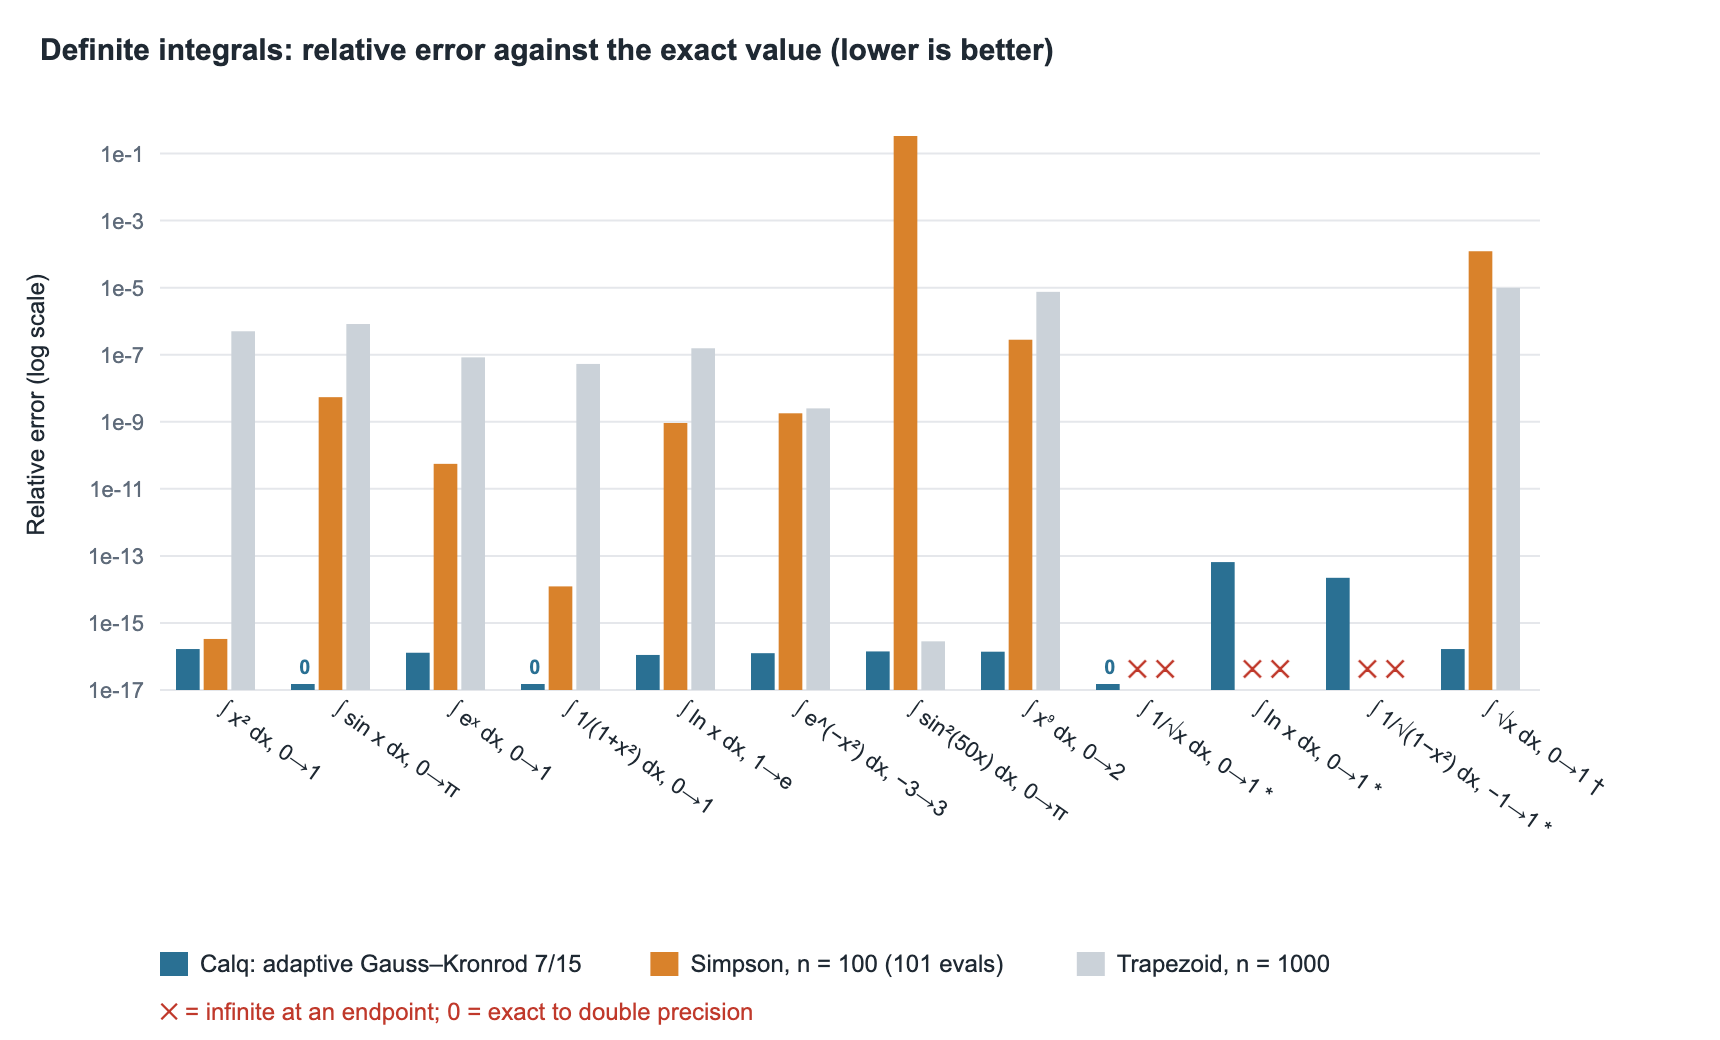
\includegraphics[width=13.5cm]{figures/bench_integration.png}
\figcaption{Figure 6.1: Relative error of Calq’s adaptive Gauss–Kronrod quadrature against Simpson’s and the trapezoidal rule (* singular at an endpoint, † kink at 0)}{Figure 6.1: Relative error of Calq’s adaptive Gauss–Kronrod quadrature against Simpson’s and the trapezoidal rule (* singular at an endpoint, † kink at 0)}
\end{figblock}

Calq nailed every integral to within 6.5×10\textsuperscript{−14}, usually at the limit of double precision, with between 60 and 2790 function evaluations. Simpson’s rule with a comparable 101 evaluations is excellent on smooth polynomials but cannot evaluate the three singular integrals at all (f is infinite at the endpoint), is accurate only to about 10\textsuperscript{−4} on √x because of its kink at 0, and is wrong by 3.3×10\textsuperscript{−1} on sin²(50x): with 100 intervals over 50 periods its samples alias with the oscillation. The adaptive method detects this from its error estimate and spends 2790 evaluations there instead of 60.

\Htwo{6.4 Derivatives against a single central difference}{6.4 Derivatives against a single central difference}

\begin{figblock}
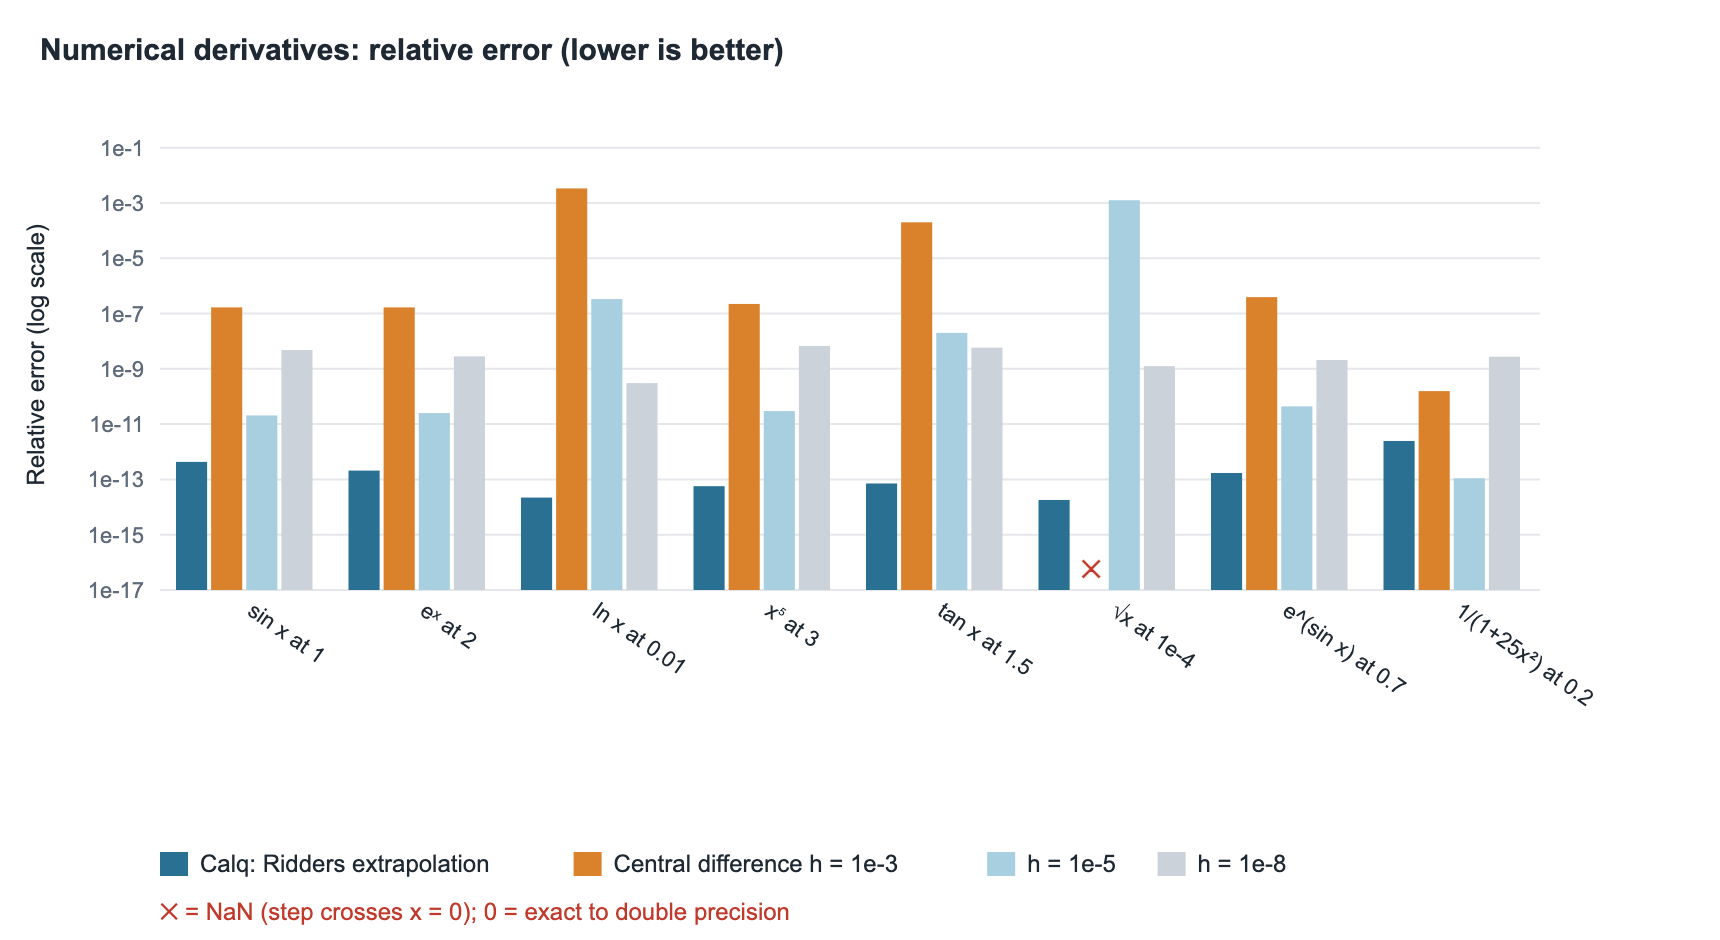
\includegraphics[width=13.5cm]{figures/bench_deriv.png}
\figcaption{Figure 6.2: Relative error of Ridders’ extrapolation against a single central difference with three step sizes}{Figure 6.2: Relative error of Ridders’ extrapolation against a single central difference with three step sizes}
\end{figblock}

Ridders’ method was below 2.5×10\textsuperscript{−12} at all eight points. No single step size for the central difference comes close: h = 10\textsuperscript{−3} has truncation errors up to 3×10\textsuperscript{−3} (ln x at 0.01), h = 10\textsuperscript{−8} is dominated by rounding error at around 10\textsuperscript{−9}, and h = 10\textsuperscript{−5}, the best compromise, still reaches 1.3×10\textsuperscript{−3} on √x near 0, where h = 10\textsuperscript{−3} fails outright because x − h is negative. The extrapolation removes the need to choose h, which is exactly the decision a calculator user cannot make.

\Htwo{6.5 ODEs against RK4 and Euler}{6.5 ODEs against RK4 and Euler}

\begin{figblock}
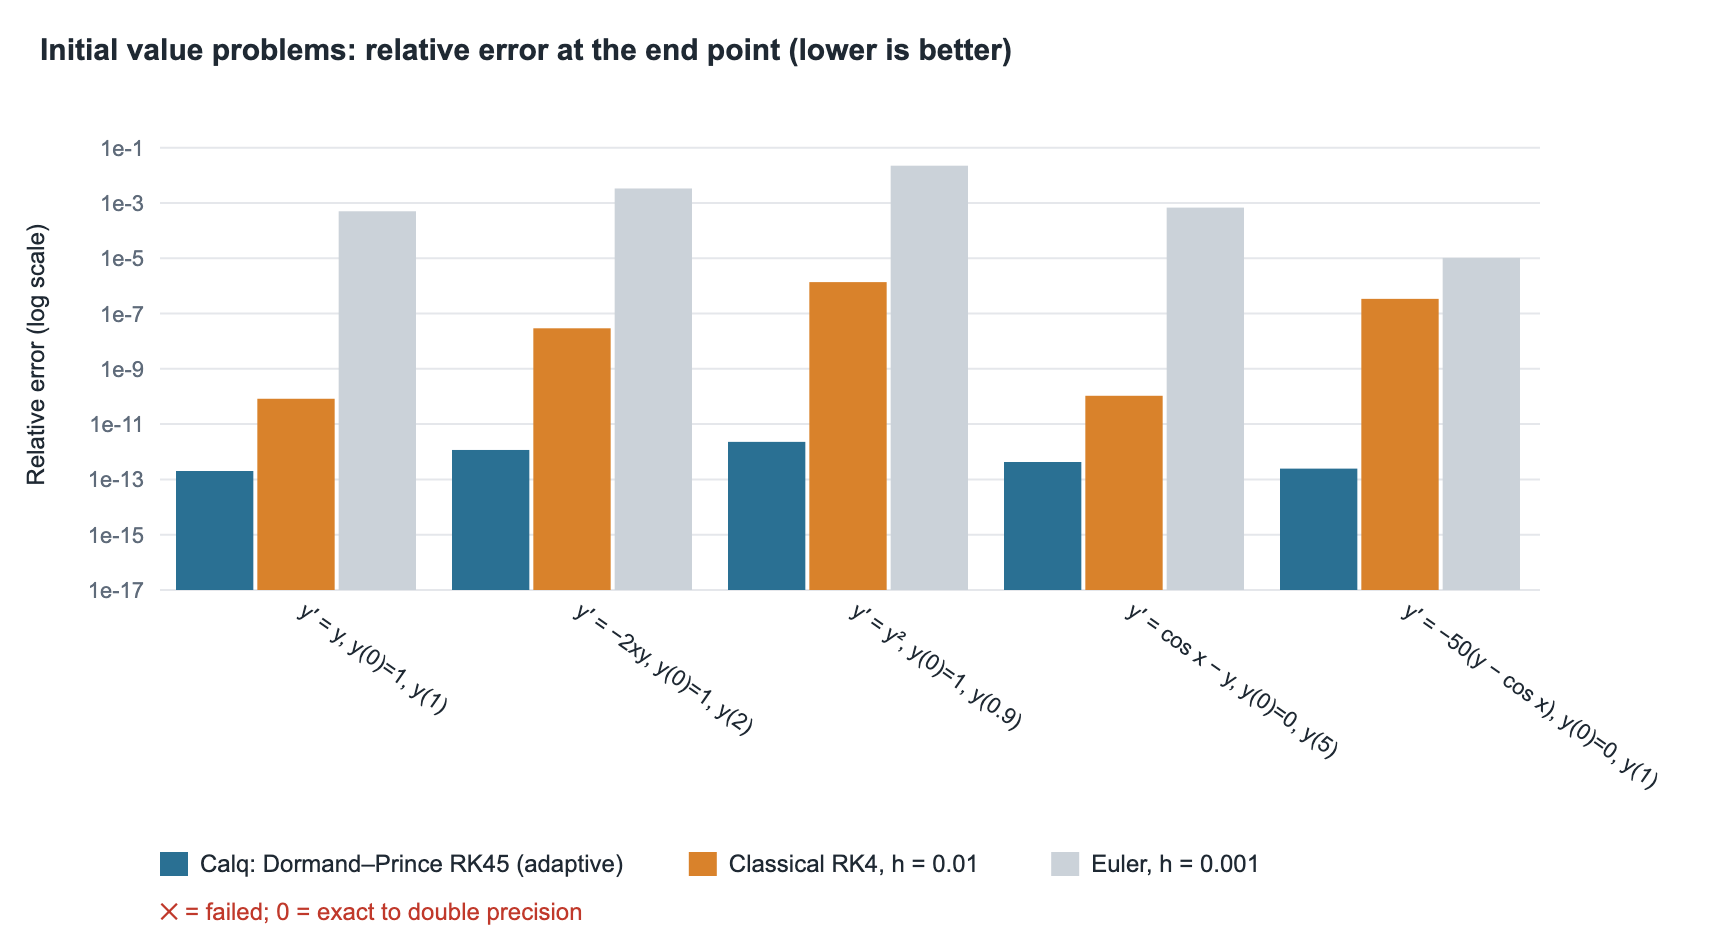
\includegraphics[width=13.5cm]{figures/bench_ode.png}
\figcaption{Figure 6.3: Relative error at the end point for Dormand–Prince (adaptive), classical RK4 (h = 0.01) and Euler (h = 0.001)}{Figure 6.3: Relative error at the end point for Dormand–Prince (adaptive), classical RK4 (h = 0.01) and Euler (h = 0.001)}
\end{figblock}

Dormand–Prince stayed below 2.3×10\textsuperscript{−12} on all five problems. RK4 with h = 0.01 is respectable on smooth problems but loses accuracy to 1.4×10\textsuperscript{−6} on y′ = y² as the solution approaches its blow-up at x = 1, and Euler’s errors range from 10\textsuperscript{−5} to 2.2×10\textsuperscript{−2}. Calq is two to six orders of magnitude more accurate than RK4 and up to ten more than Euler, and at about 1.5 ms per solve the user never waits.

\Htwo{6.6 Verification layer under fault injection}{6.6 Verification layer under fault injection}

\begin{figblock}
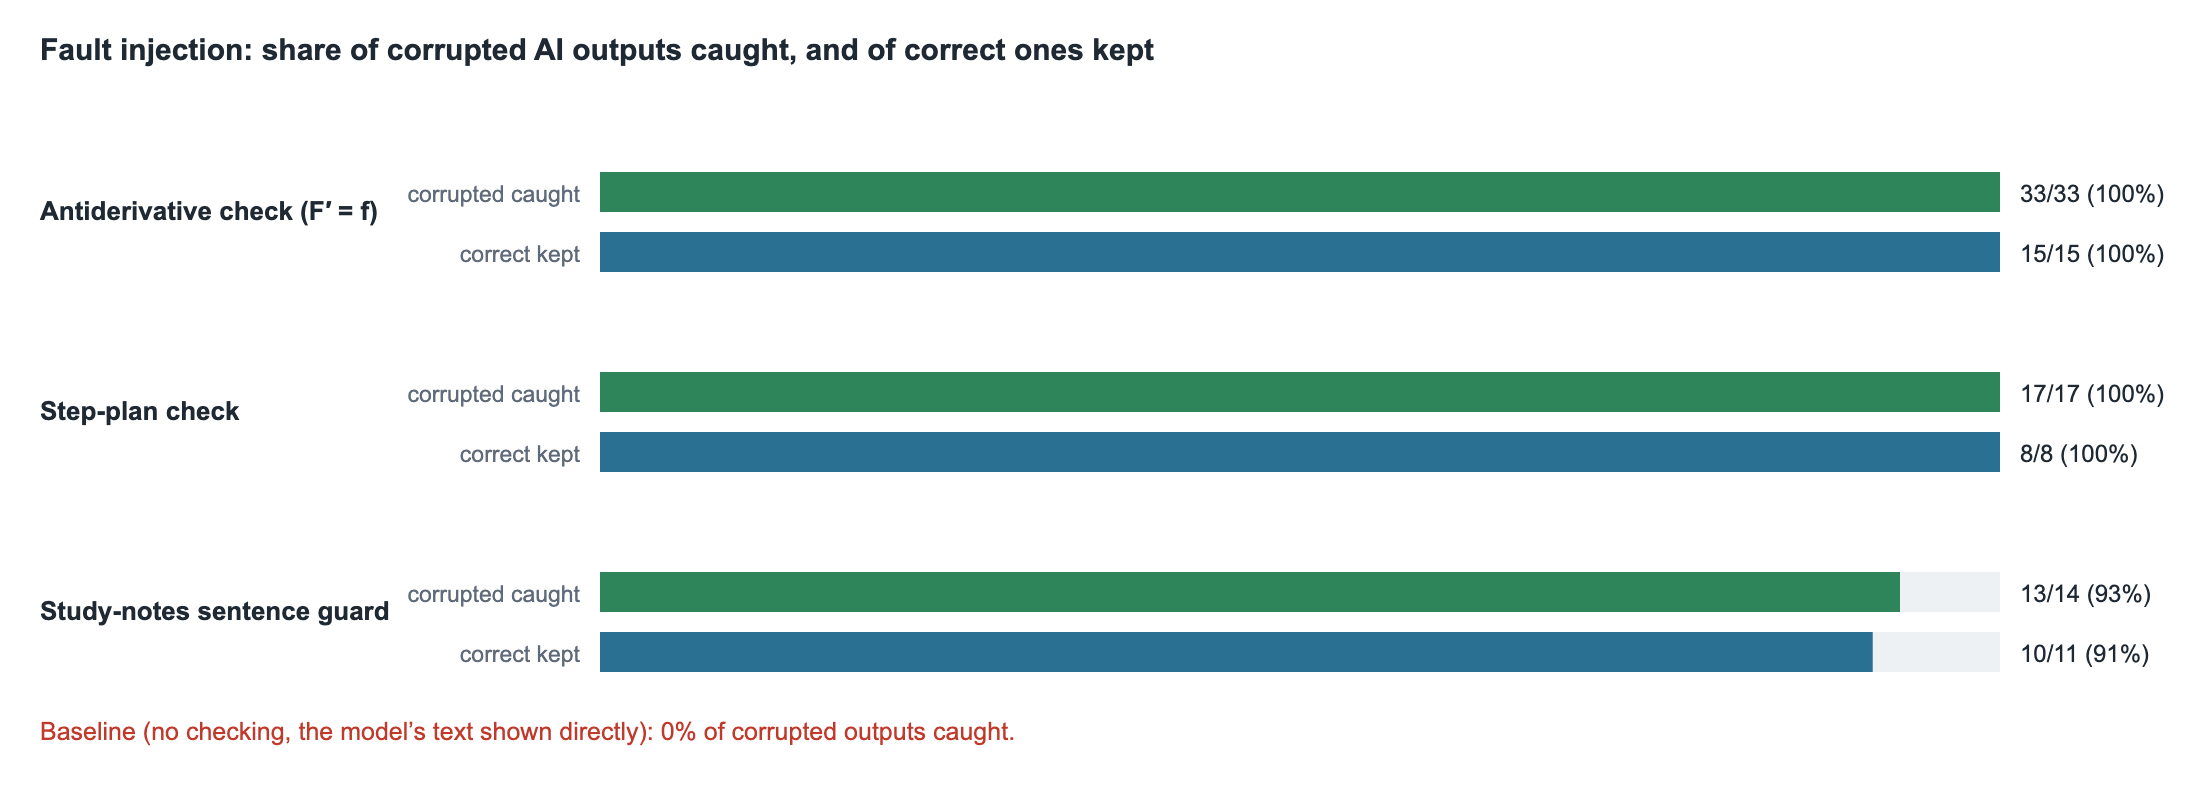
\includegraphics[width=14cm]{figures/bench_verifier.png}
\figcaption{Figure 6.4: Share of corrupted AI outputs rejected and of correct outputs accepted by each on-device checker}{Figure 6.4: Share of corrupted AI outputs rejected and of correct outputs accepted by each on-device checker}
\end{figblock}

\begin{tableblock}
\begin{tabular}{|>{\raggedright\arraybackslash}p{\dimexpr 0.3000\linewidth - 2\tabcolsep - 1.4\arrayrulewidth\relax}|>{\raggedright\arraybackslash}p{\dimexpr 0.2200\linewidth - 2\tabcolsep - 1.4\arrayrulewidth\relax}|>{\raggedright\arraybackslash}p{\dimexpr 0.2200\linewidth - 2\tabcolsep - 1.4\arrayrulewidth\relax}|>{\raggedright\arraybackslash}p{\dimexpr 0.2600\linewidth - 2\tabcolsep - 1.4\arrayrulewidth\relax}|}
\hline
\textbf{Checker} & \textbf{Corrupted caught} & \textbf{Correct kept} & \textbf{Baseline (no check) caught} \\ \hline
Antiderivative (F′ = f) & 33/33 (100\%) & 15/15 (100\%) & 0\% \\ \hline
Step plan & 17/17 (100\%) & 8/8 (100\%) & 0\% \\ \hline
Study-notes guard & 13/14 (93\%) & 10/11 (91\%) & 0\% \\ \hline
\textbf{Total} & \textbf{63/64 (98.4\%)} & \textbf{33/34 (97.1\%)} & \textbf{0\%} \\ \hline
\end{tabular}
\end{tableblock}
\tabcaption{Table 6.1: Fault-injection results by checker}{Table 6.1: Fault-injection results by checker}

The antiderivative and step-plan checkers caught every corruption, including the subtle ones: a missing 180/π factor in degree mode, a 200/π factor used where 180/π was needed, and a rewrite of 489×73 that is off by one in the units digit. They also accepted every correct answer. These checkers compare numbers that the app computes itself, so they have no blind spots within their tolerance.

The study-notes guard, which works on free-form prose rather than numbers, still caught 13 of 14 corrupted sentences and kept 10 of 11 correct ones. When in doubt it deletes a sentence rather than risk a wrong one, so the notes stay trustworthy.

\Htwo{6.7 Local steps}{6.7 Local steps}

Every one of the 20 multi-operation test expressions produced checked steps on the device (2 to 5 lines each, counting the expression itself), in at most about 1 ms, including the precedence cases 6÷2(1+2) and −3²+4 that students most often get wrong. As a result the AI is now asked only for shortcuts on hard arithmetic such as 489×73, which cut AI calls for steps to a small fraction of what the first version made and let guests use Steps without an account.

\Htwo{6.8 Performance}{6.8 Performance}

\begin{figblock}
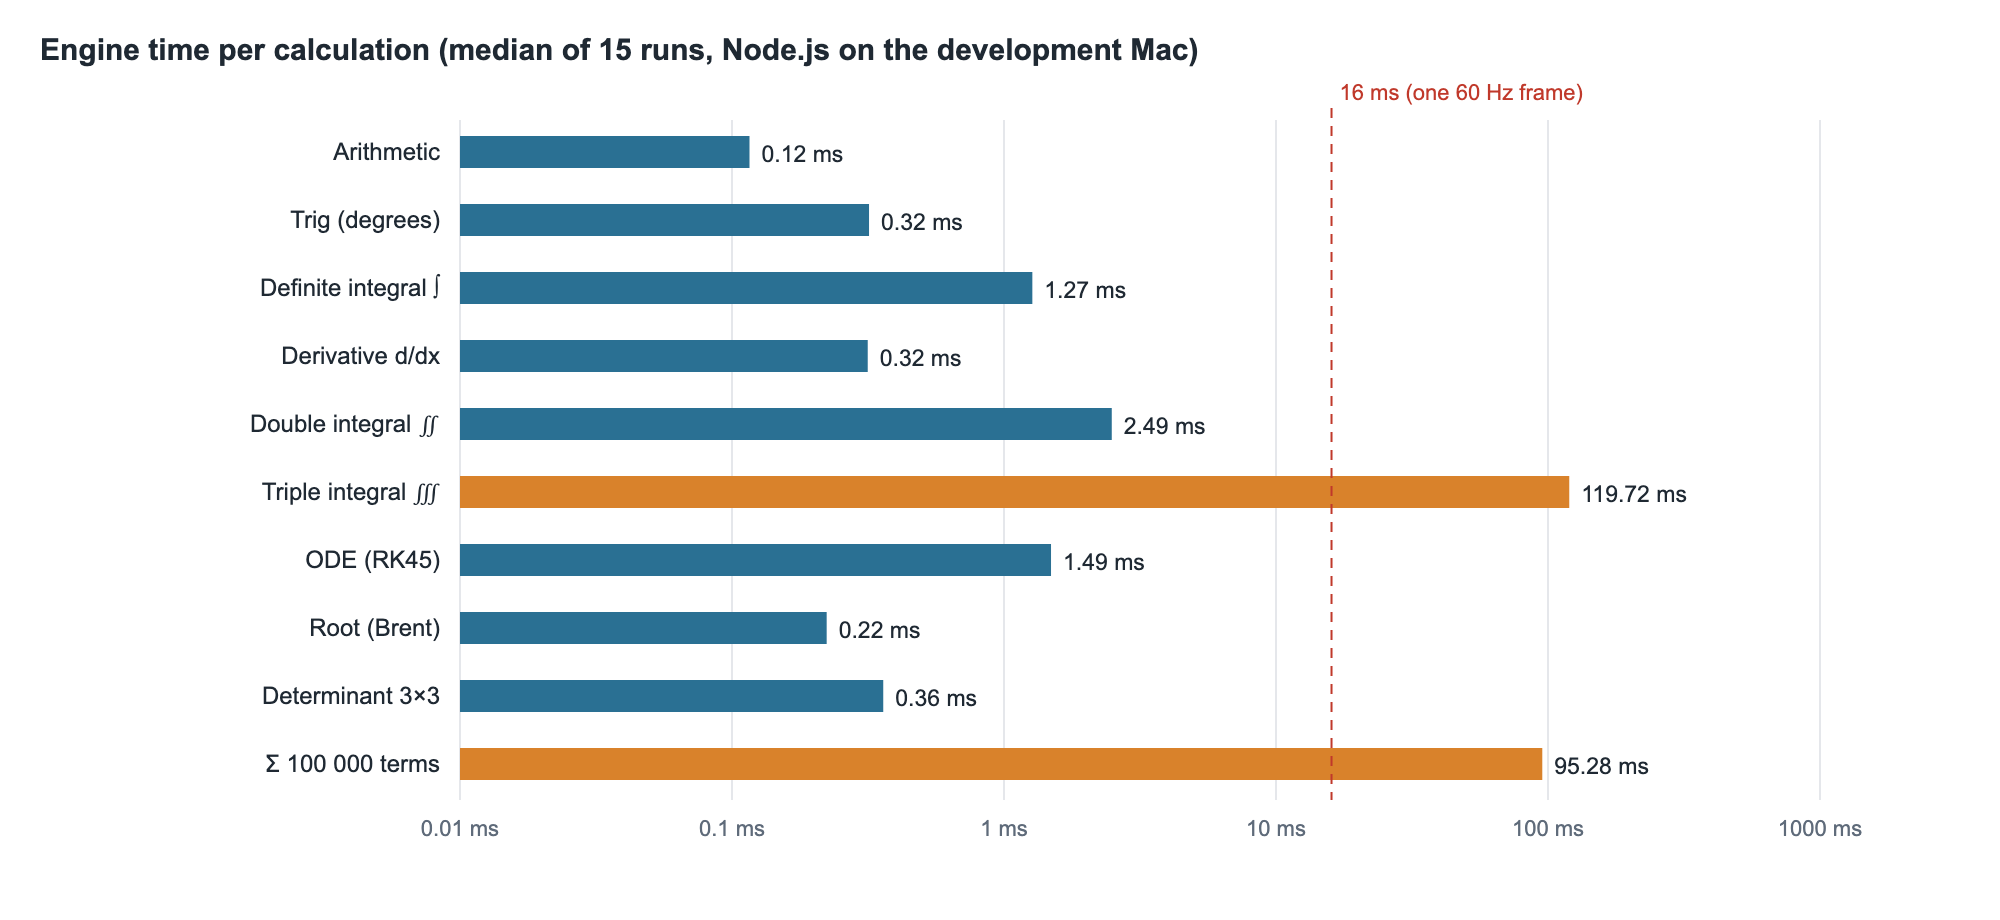
\includegraphics[width=12.5cm]{figures/bench_latency.png}
\figcaption{Figure 6.5: Median engine time per calculation class}{Figure 6.5: Median engine time per calculation class}
\end{figblock}

Eight of the ten calculation classes finish in under 3 ms (median), comfortably inside one 60 Hz frame. The two slow cases are the triple integral (120 ms; three nested adaptive integrations) and Σ over 100,000 terms (95 ms). Both are flagged as slow keys: they skip the live preview and show “Working it out…” instead of freezing the keypad. Because of that, the keypad never freezes, even on slower phones.

\Htwo{6.9 Every objective met}{6.9 Every objective met}

\begin{tableblock}
\begin{tabular}{|>{\raggedright\arraybackslash}p{\dimexpr 0.0700\linewidth - 2\tabcolsep - 1.4\arrayrulewidth\relax}|>{\raggedright\arraybackslash}p{\dimexpr 0.2800\linewidth - 2\tabcolsep - 1.4\arrayrulewidth\relax}|>{\raggedright\arraybackslash}p{\dimexpr 0.4900\linewidth - 2\tabcolsep - 1.4\arrayrulewidth\relax}|>{\raggedright\arraybackslash}p{\dimexpr 0.1600\linewidth - 2\tabcolsep - 1.4\arrayrulewidth\relax}|}
\hline
\textbf{ID} & \textbf{Target} & \textbf{Result} & \textbf{Status} \\ \hline
O1 & Reference set within 10\textsuperscript{−8} & 40/40 (100\%); worst error 1.2×10\textsuperscript{−12} & Met \\ \hline
O2 & AI outputs checked; ≥ 90\% caught; ≥ 90\% kept & 4 of 4 AI paths checked; 63/64 (98.4\%) caught; 33/34 (97.1\%) kept & Met \\ \hline
O3 & Local steps for all multi-operation tests & 20/20 expressions & Met \\ \hline
O4 & Typical calculation < 16 ms; slow keys show progress & 8 of 10 classes < 3 ms; ∫∫∫ 120 ms and Σ of 10\textsuperscript{5} terms 95 ms show “Working it out…” & Met \\ \hline
O5 & Rules tests pass; sync works & 16/16 rules tests; two-device sync checked manually & Met \\ \hline
O6 & All tests pass; ≥ 80\% lines; no lint errors & 546/546 pass; 92.1\% lines; 0 lint errors & Met \\ \hline
O7 & SGD 0 spend; builds before Week 12 & SGD 0 hardware/software \fillin{[CONFIRM AI API spend]}; iOS and Android builds in Week 10 & Met \fillin{[CONFIRM]} \\ \hline
\end{tabular}
\end{tableblock}
\tabcaption{Table 6.2: Results against the objectives of Table 1.1}{Table 6.2: Results against the objectives of Table 1.1}

\clearpage
\Hone{7. Project Management}{7. Project Management}

\Htwo{7.1 Team and roles}{7.1 Team and roles}

\begin{tableblock}
\begin{tabular}{|>{\raggedright\arraybackslash}p{\dimexpr 0.2600\linewidth - 2\tabcolsep - 1.4\arrayrulewidth\relax}|>{\raggedright\arraybackslash}p{\dimexpr 0.3000\linewidth - 2\tabcolsep - 1.4\arrayrulewidth\relax}|>{\raggedright\arraybackslash}p{\dimexpr 0.4400\linewidth - 2\tabcolsep - 1.4\arrayrulewidth\relax}|}
\hline
\textbf{Member} & \textbf{Role} & \textbf{Main responsibilities} \\ \hline
Ong Dun Yan & Project manager; frontend and Firebase backend & Planning and coordination; app architecture; calculator UI; Firestore, rules and sync; exports and Drive; advanced maths engine; verification layer; tests and README \\ \hline
Chan Wei Kiat & Treasurer; UI/UX design & Budget tracking and claims; Claude Design screens and visual style \\ \hline
Emerson Jebadurai Joel & LLM and OCR & First Cloud Functions for scan and AI steps; step-plan retry; prompt design \\ \hline
Lee Jie Xuan Gina & UI/UX design & Claude Design layouts and user flows \fillin{[CONFIRM]} \\ \hline
Nathaniel Naveen Umaibalan & UI/UX design & Claude Design keypad layouts and mock-ups (Figure 4.1) \fillin{[CONFIRM]} \\ \hline
Naili Naufal Bin Abdul Rashid & OCR & Scan transcription rules and photo test cases \fillin{[CONFIRM]} \\ \hline
\end{tabular}
\end{tableblock}
\tabcaption{Table 7.1: Team members and roles}{Table 7.1: Team members and roles}

We met every Wednesday from 1.30 pm to 4.30 pm in our assigned lab, Information Systems (S2-B3a-06), as the course requires, and used the first part of each session for a short round of updates against the plan. Between sessions we coordinated in a group chat \fillin{[FILL IN: platform]} and through GitHub. Work that touched several areas went on a feature branch (for example feat/keyboard, feat/unit-options, feat/export) and was merged through a pull request, with commit messages in the Conventional Commits style (feat(math): …, fix(history): …) so that the history doubles as a change log. The README was kept current so that any member could build and run the app from a fresh clone.

\Htwo{7.2 Schedule: planned against actual}{7.2 Schedule: planned against actual}

Figure 7.1 compares the charter’s schedule with what happened. Academic weeks are those of Semester 1, AY2026/27, with the recess week between Weeks 7 and 8.

\begin{figblock}
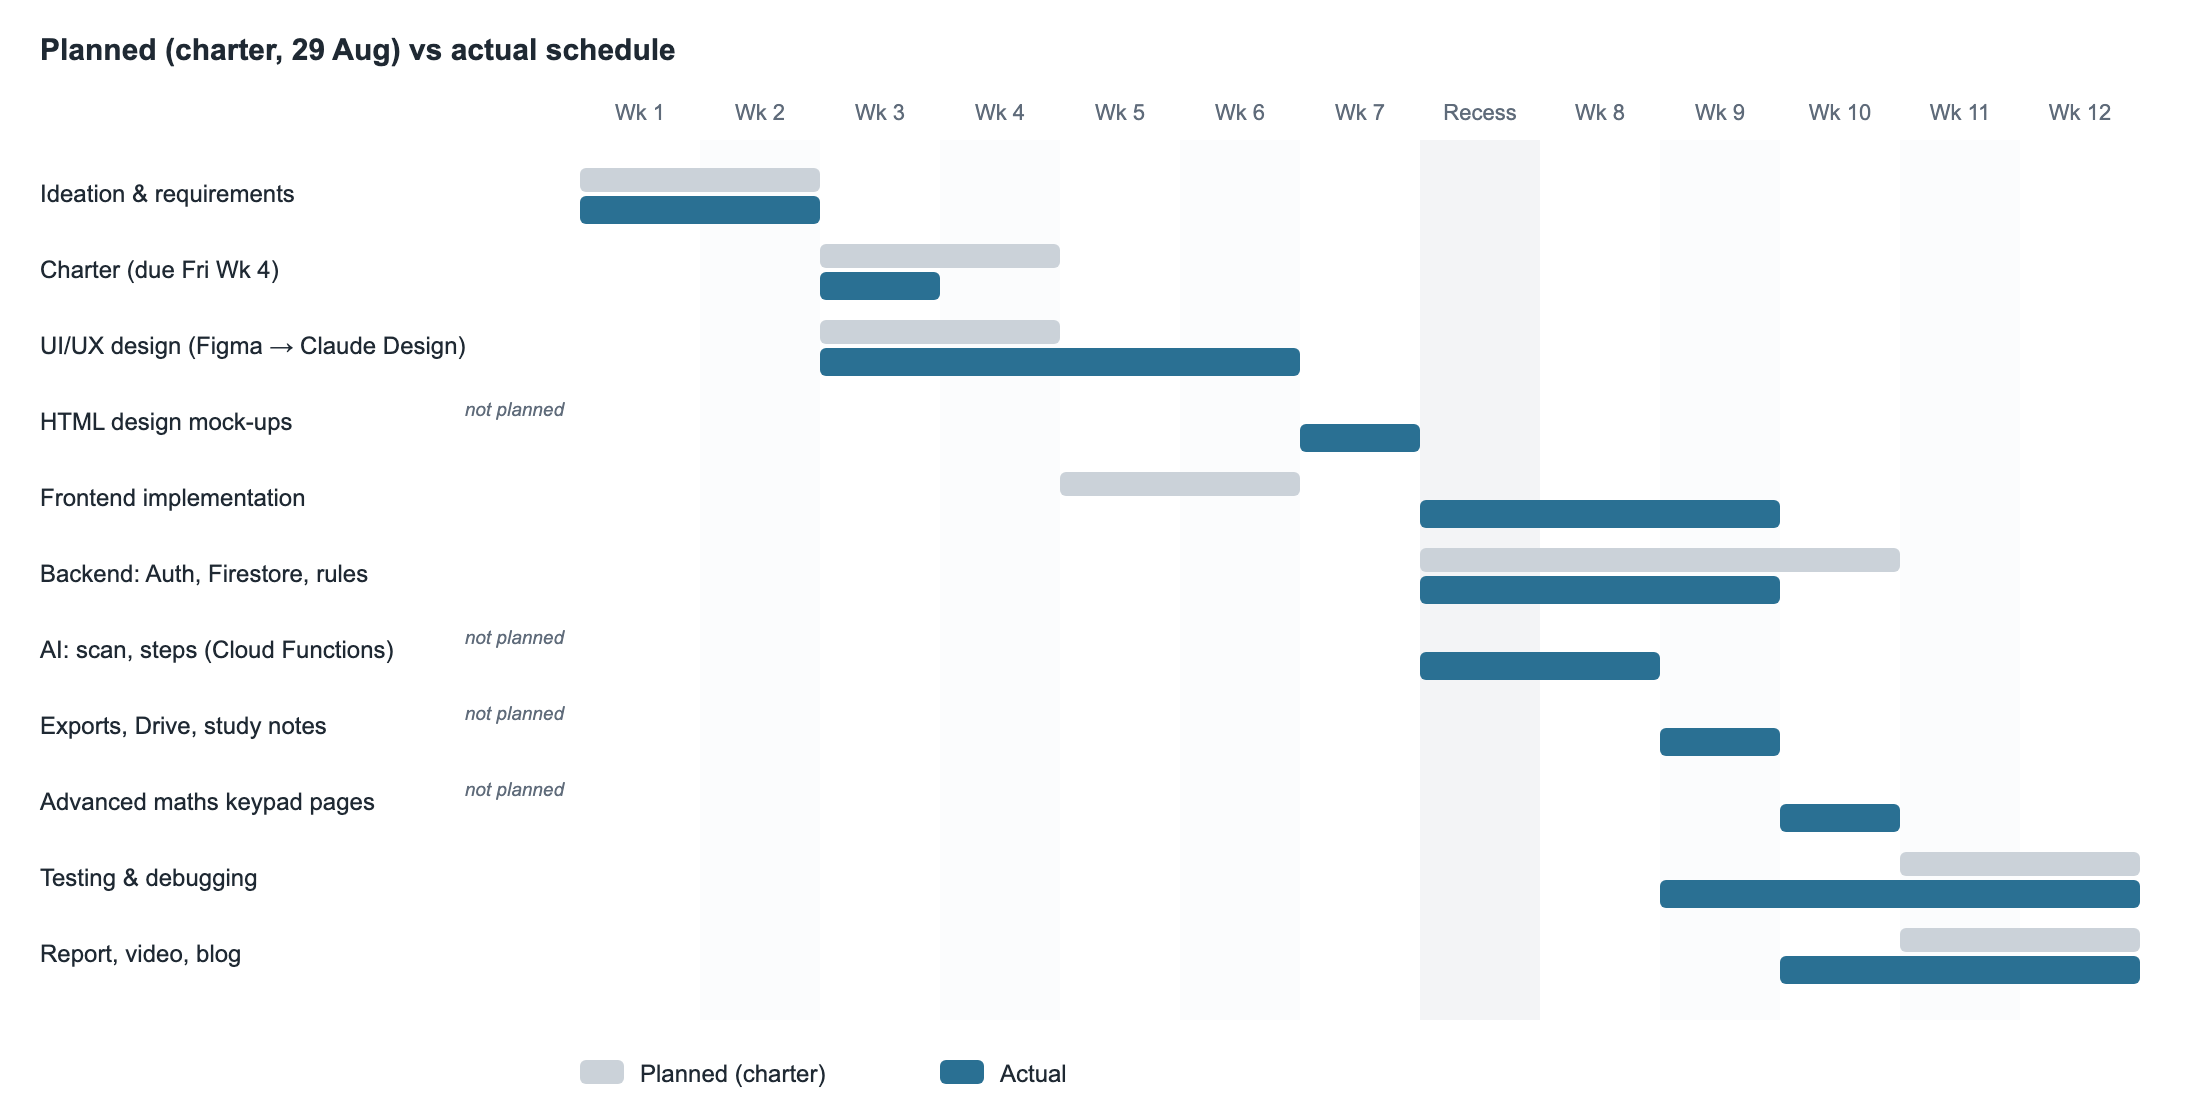
\includegraphics[width=15.9cm]{figures/gantt.png}
\figcaption{Figure 7.1: Planned (charter) and actual schedule}{Figure 7.1: Planned (charter) and actual schedule}
\end{figblock}

\begin{tableblock}
\begin{tabular}{|>{\raggedright\arraybackslash}p{\dimexpr 0.2400\linewidth - 2\tabcolsep - 1.4\arrayrulewidth\relax}|>{\raggedright\arraybackslash}p{\dimexpr 0.1800\linewidth - 2\tabcolsep - 1.4\arrayrulewidth\relax}|>{\raggedright\arraybackslash}p{\dimexpr 0.1800\linewidth - 2\tabcolsep - 1.4\arrayrulewidth\relax}|>{\raggedright\arraybackslash}p{\dimexpr 0.4000\linewidth - 2\tabcolsep - 1.4\arrayrulewidth\relax}|}
\hline
\textbf{Activity} & \textbf{Planned} & \textbf{Actual} & \textbf{Cause and effect} \\ \hline
UI/UX design & Weeks 3–4 (Figma) & Weeks 3–7 (Claude Design) & Design moved from Figma to Claude Design, went through more iterations than planned and overlapped mid-semester tests; it pushed the start of coding back by three weeks \\ \hline
Frontend implementation & Weeks 5–6 & Weeks 8–9 & Started after the HTML mock-ups were agreed in the recess week; recovered time by building frontend and backend in parallel \\ \hline
Backend & Weeks 7–9 & Weeks 8–9 & Firebase’s managed services (Auth, Firestore, Functions) needed far less code than a custom server; finished a week early \\ \hline
AI features, exports, Drive & Not planned & Weeks 8–9 & Added scope (§3.3), made possible by the fast backend \\ \hline
Advanced maths pages & Not planned & Week 10 & Added scope; built test-first to limit risk late in the project \\ \hline
Testing and debugging & Weeks 10–12 & Weeks 9–12 & Started earlier because tests were written alongside features \\ \hline
Report, video and blog & Weeks 10–12 & Weeks 10–12 & As planned \fillin{[CONFIRM after Week 12]} \\ \hline
\end{tabular}
\end{tableblock}
\tabcaption{Table 7.2: Schedule variances and their causes}{Table 7.2: Schedule variances and their causes}

We invested extra weeks in design up front, and it paid off: once the layouts were settled, building on managed services and running frontend, backend and AI work in parallel took the app from first commit to feature-complete in about three weeks, with scope well beyond the charter.

\Htwo{7.3 Budget: planned against actual}{7.3 Budget: planned against actual}

The charter planned a budget of SGD 0, well within the course limit of SGD 1,000 per project. Table 7.3 lists every cost item.

\begin{tableblock}
\begin{tabular}{|>{\raggedright\arraybackslash}p{\dimexpr 0.3600\linewidth - 2\tabcolsep - 1.4\arrayrulewidth\relax}|>{\raggedright\arraybackslash}p{\dimexpr 0.1400\linewidth - 2\tabcolsep - 1.4\arrayrulewidth\relax}|>{\raggedright\arraybackslash}p{\dimexpr 0.1800\linewidth - 2\tabcolsep - 1.4\arrayrulewidth\relax}|>{\raggedright\arraybackslash}p{\dimexpr 0.3200\linewidth - 2\tabcolsep - 1.4\arrayrulewidth\relax}|}
\hline
\textbf{Item} & \textbf{Planned} & \textbf{Actual} & \textbf{Note} \\ \hline
Development hardware (laptops, phones) & 0 & 0 & Members’ own devices \\ \hline
Expo, React Native, math.js, GitHub, Claude Design & 0 & \fillin{[CONFIRM]} & Free and open-source tools; Claude Design under an existing Claude plan \fillin{[CONFIRM]} \\ \hline
Firebase (Auth, Firestore, Cloud Functions) & 0 & \fillin{[FILL IN]} & Blaze pay-as-you-go plan is required for Cloud Functions; usage stayed within the free allowance \fillin{[CONFIRM]} \\ \hline
AI model API (OpenRouter) & 0 & \fillin{[FILL IN]} & Pay per token; daily quotas cap the worst case \\ \hline
Apple Developer Program / Google Play & 0 & 0 & Not needed: development builds and APK sharing \\ \hline
\textbf{Total} & \textbf{0} & \textbf{[FILL IN]} & Within the SGD 1,000 course limit \\ \hline
\end{tabular}
\end{tableblock}
\tabcaption{Table 7.3: Budget planned against actual (SGD)}{Table 7.3: Budget planned against actual (SGD)}

The AI features are the only variable cost. We controlled it in the design rather than by monitoring alone: steps are computed on the device and the AI is asked only for shortcuts on hard arithmetic, photos are compressed to about 200 KB before upload, and each user has daily quotas (§4.6.2).

\Htwo{7.4 Risk management}{7.4 Risk management}

The charter named three high-level risks: the learning curve, integration difficulty and budget limits. We expanded them into a register (Table 7.4), scored each by likelihood and impact on a 1–5 scale, and reviewed it at the weekly meeting. Figure 7.2 places the risks on a matrix before mitigation.

\begin{figblock}
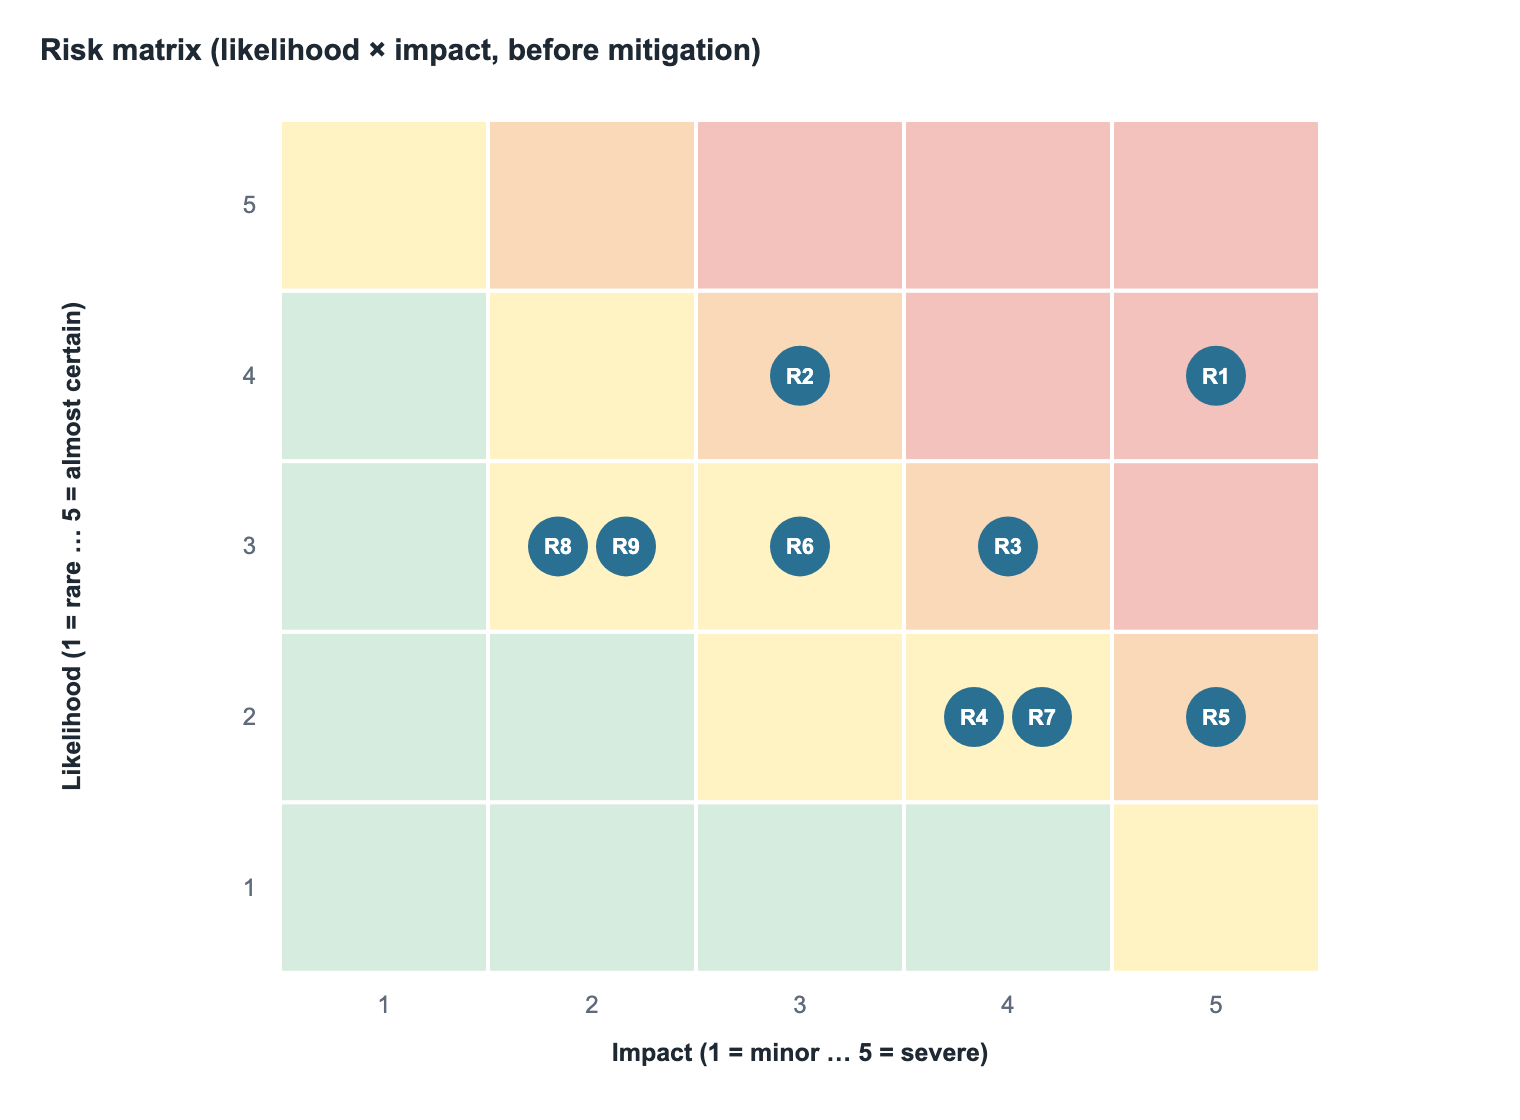
\includegraphics[width=9cm]{figures/risk_matrix.png}
\figcaption{Figure 7.2: Risk matrix before mitigation (risk IDs refer to Table 7.4)}{Figure 7.2: Risk matrix before mitigation (risk IDs refer to Table 7.4)}
\end{figblock}

\begin{tableblock}
\begin{tabular}{|>{\raggedright\arraybackslash}p{\dimexpr 0.0600\linewidth - 2\tabcolsep - 1.4\arrayrulewidth\relax}|>{\raggedright\arraybackslash}p{\dimexpr 0.2200\linewidth - 2\tabcolsep - 1.4\arrayrulewidth\relax}|>{\raggedright\arraybackslash}p{\dimexpr 0.0600\linewidth - 2\tabcolsep - 1.4\arrayrulewidth\relax}|>{\raggedright\arraybackslash}p{\dimexpr 0.0600\linewidth - 2\tabcolsep - 1.4\arrayrulewidth\relax}|>{\raggedright\arraybackslash}p{\dimexpr 0.0600\linewidth - 2\tabcolsep - 1.4\arrayrulewidth\relax}|>{\raggedright\arraybackslash}p{\dimexpr 0.3200\linewidth - 2\tabcolsep - 1.4\arrayrulewidth\relax}|>{\raggedright\arraybackslash}p{\dimexpr 0.2200\linewidth - 2\tabcolsep - 1.4\arrayrulewidth\relax}|}
\hline
\textbf{ID} & \textbf{Risk} & \textbf{L} & \textbf{I} & \textbf{L×I} & \textbf{Mitigation} & \textbf{Outcome} \\ \hline
R1 & LLM returns wrong maths & 4 & 5 & 20 & Verify-first design; model never supplies shown numbers; fault-injection tests & Occurred in testing; every case caught or safely dropped \\ \hline
R2 & Learning curve (React Native, Firebase) & 4 & 3 & 12 & One language (JS) for all; README with exact setup; pair debugging in lab sessions & Partly occurred; slowed early weeks \\ \hline
R3 & Toolchain version lock (Expo, Xcode, JDK) & 3 & 4 & 12 & Pinned Expo SDK 55; documented JDK 17 for Android and Java 21 for the emulator & Occurred; resolved within a day each time \\ \hline
R4 & AI cost exceeds budget & 2 & 4 & 8 & Local steps, image compression, per-user daily quotas, cheap open-weights models & Did not occur \fillin{[CONFIRM]} \\ \hline
R5 & API key or user data exposed & 2 & 5 & 10 & Key as server secret; owner-only rules with 16 tests; drive.file scope & Did not occur \\ \hline
R6 & Late integration of features & 3 & 3 & 9 & Feature branches, pull requests, tests alongside features & Minor merge conflicts only \\ \hline
R7 & Sync conflicts or data loss offline & 2 & 4 & 8 & Local-first history, UUID document ids, idempotent merge & Occurred once (offline start); fixed (§4.7) \\ \hline
R8 & Design and code drift apart & 3 & 2 & 6 & HTML mock-ups agreed before coding; shared colour tokens & Controlled \\ \hline
R9 & Member availability (tests, other projects) & 3 & 2 & 6 & Weekly check-in; tasks sized to one week & Design overran by three weeks (§7.2) \\ \hline
\end{tabular}
\end{tableblock}
\tabcaption{Table 7.4: Risk register}{Table 7.4: Risk register}

\Hone{8. Key Learnings and What’s Next}{8. Key Learnings and What’s Next}

\Htwo{8.1 What made Calq work}{8.1 What made Calq work}

\begin{itemize}
\item \textbf{Verify, don’t trust.} Deciding early that the model may never supply a number made every AI feature safe by construction, and let us use fast, low-cost open-weights models.
\item \textbf{AI only where it adds value.} Ordinary steps are computed instantly on the phone, for everyone, offline. The model is saved for what people find genuinely hard: shortcuts through big arithmetic, reading photos and writing explanations.
\item \textbf{A managed backend.} Firebase gave us sign-in, a synced database with offline support and tested access control in a few hundred lines, freeing the team to focus on the maths and the experience.
\item \textbf{Tests alongside features.} Every feature shipped with its tests, so late additions such as gradians and the advanced keypad pages never broke earlier work.
\end{itemize}

\Htwo{8.2 Challenges we solved}{8.2 Challenges we solved}

\Hthree{8.2.1 Making working fast and free}{8.2.1 Making working fast and free}

The first Steps feature asked the AI for every calculation, which took seconds and needed an account. We built an on-device engine (localSteps) that produces checked steps in about a millisecond for anyone, and kept the AI for the arithmetic shortcuts it is best at.

\Hthree{8.2.2 Taming the toolchain}{8.2.2 Taming the toolchain}

Expo, Xcode and the Android build each need specific versions: Expo SDK 55 with Xcode 26.3, JDK 17 for Android builds and Java 21 for the Firestore emulator, plus each member’s signing fingerprint for Google sign-in. We pinned and documented every version in the README, so any member can build the app from a fresh clone.

\Hthree{8.2.3 Reliable offline sync}{8.2.3 Reliable offline sync}

Starting the app offline could briefly show an empty history from Firestore’s cache. Calq now waits for the server before trusting an empty list and keeps its own copy on the device, so history is always there, online or not.

\Hthree{8.2.4 Room for big results}{8.2.4 Room for big results}

When the advanced keys arrived, matrix and SVD results outgrew the original 200-character limit in the security rules. We raised it to 2,000 characters and added boundary tests, so large results sync as reliably as small ones.

\Htwo{8.3 What’s next}{8.3 What’s next}

\begin{itemize}
\item \textbf{Graphing} of functions and ODE solutions, reusing the numerical engine that already exists.
\item \textbf{A scan benchmark} of about 100 labelled photos from NTU tutorial sheets and handwritten notes, to tune the scan prompt further.
\item \textbf{Even sharper notes,} by tightening how the guard reads claims and counting words.
\item \textbf{Self-hosted models:} the provider is a single setting, so Qwen3 could run on school GPUs with no code changes.
\item \textbf{App Store and Google Play release,} after a usability study with classmates.
\end{itemize}

\Hone{9. Individual Contributions}{9. Individual Contributions}

Each subsection was written by or agreed with the member concerned, and matches their progress blog. Appendix A summarises the contributions with signatures.

\Htwo{9.1 Ong Dun Yan (project manager; frontend and Firebase backend)}{9.1 Ong Dun Yan (project manager; frontend and Firebase backend)}

I led planning, the weekly meetings and the GitHub workflow, and was responsible for the app’s architecture and most of its code: the calculator screen and keypad pages, the expression pipeline and maths engine including the advanced numerical methods, history with Firestore sync and offline handling, security rules and their emulator tests, exports and the Google Drive integration, the verification layer for AI output (local steps, the antiderivative check and the study-notes guard) and the README. The hardest problem was making AI help trustworthy; the answer, never letting the model supply a number, became the theme of the project. \fillin{[FILL IN: personal reflection, 3{–}5 sentences]}

\Htwo{9.2 Chan Wei Kiat (treasurer; UI/UX design)}{9.2 Chan Wei Kiat (treasurer; UI/UX design)}

As treasurer I tracked the budget against the charter and handled claims \fillin{[FILL IN: details]}. As part of the design team I worked on the Claude Design screens and the visual style that the app uses: the blue palette, the paged keypad and the history layout \fillin{[CONFIRM: specific screens]}. \fillin{[FILL IN: personal reflection]}

\Htwo{9.3 Emerson Jebadurai Joel (LLM and OCR)}{9.3 Emerson Jebadurai Joel (LLM and OCR)}

I built the first AI features as Firebase Cloud Functions: scanEquation, which reads a problem from a photo, and explainSteps, which plans step-by-step working, together with the app code that checks a step plan and retries a rejected one, and broke hard arithmetic into partial products so that a person can follow it (pull request \#1). \fillin{[FILL IN: prompt iterations, model choice, personal reflection]}

\Htwo{9.4 Lee Jie Xuan Gina (UI/UX design)}{9.4 Lee Jie Xuan Gina (UI/UX design)}

\fillin{[FILL IN: Claude Design layouts, user flows, mock-ups or other design work, with the figures or blog posts that show it; personal reflection]}

\Htwo{9.5 Nathaniel Naveen Umaibalan (UI/UX design)}{9.5 Nathaniel Naveen Umaibalan (UI/UX design)}

\fillin{[FILL IN: design work in Claude Design, e.g. the numeric and scientific keypad layouts of Figure 4.1(a), mock-ups; personal reflection]}

\Htwo{9.6 Naili Naufal Bin Abdul Rashid (OCR)}{9.6 Naili Naufal Bin Abdul Rashid (OCR)}

\fillin{[FILL IN: OCR work, e.g. collecting test photos, refining the transcription rules in the scan prompt, testing handwriting; personal reflection]}

\Hone{10. Conclusion}{10. Conclusion}

Calq set out to be a better scientific calculator for students: one that remembers, syncs and exports their work. It is that, and it also answers a question that matters more every year: how to use AI in a tool whose whole purpose is to be right. By letting the model propose structure and requiring the phone to check every value and claim, Calq caught 98.4\% of corrupted AI outputs in our tests while keeping 97.1\% of correct ones, where showing the model’s text directly would have caught none. Its on-device numerical methods were orders of magnitude more accurate than the simple alternatives on the same problems, and all 546 automated tests pass.

Calq delivered everything the charter promised, cloud-synced history, sign-in and rich exports, and then went further, with university-level maths on the phone and AI help students can trust. It is ready for graphing, a wider scan benchmark and a store release next.

\Hone{11. Declaration of Use of Generative AI}{11. Declaration of Use of Generative AI}

Please refer to NTU’s current policy and guidelines on the use of generative AI tools, available on the NTULearn home page.

I, \fillin{[FILL IN name]} (\fillin{[FILL IN NTU email]}), on behalf of Group E018, declare the following in relation to this submission for EE3180 Design and Innovation Project:

\begin{itemize}
\item Generative AI tools used: Claude Design (Anthropic), for the interface layouts and HTML mock-ups in §4.1; \fillin{[FILL IN any other tools and versions]}
\item Purpose: \fillin{[FILL IN, e.g. code assistance, drafting and editing of report text, generation of figures]}
\item A digital paper trail of prompts and outputs has been kept and is available on request \fillin{[FILL IN location]}.
\item Where generative AI assistance has been used, the group has reviewed, verified and takes responsibility for the content.
\end{itemize}

Note that the Calq app itself calls language models at run time (Qwen3, through OpenRouter); this is part of the product, is described in §4.5, and is distinct from any use of generative AI in preparing this report.

Signature: \_\_\_\_\_\_\_\_\_\_\_\_\_\_\_\_\_\_\_\_     Date: \_\_\_\_\_\_\_\_\_\_\_\_\_\_\_\_\_\_\_\_

\Hone{12. References}{12. References}

{\raggedright\hangindent=0.95cm\hangafter=1 Aberth, O. (1973). Iteration methods for finding all zeros of a polynomial simultaneously. \textit{Mathematics of Computation, 27}(122), 339–344.\par}

{\raggedright\hangindent=0.95cm\hangafter=1 Brent, R. P. (1973). \textit{Algorithms for minimization without derivatives}. Prentice-Hall.\par}

{\raggedright\hangindent=0.95cm\hangafter=1 Cormen, T. H., Leiserson, C. E., Rivest, R. L., \& Stein, C. (2022). \textit{Introduction to algorithms} (4th ed.). MIT Press.\par}

{\raggedright\hangindent=0.95cm\hangafter=1 de Jong, J. (2024). \textit{math.js: An extensive math library for JavaScript and Node.js} [Computer software]. \url{https://mathjs.org}\par}

{\raggedright\hangindent=0.95cm\hangafter=1 Dormand, J. R., \& Prince, P. J. (1980). A family of embedded Runge–Kutta formulae. \textit{Journal of Computational and Applied Mathematics, 6}(1), 19–26.\par}

{\raggedright\hangindent=0.95cm\hangafter=1 Edmonds, J., \& Karp, R. M. (1972). Theoretical improvements in algorithmic efficiency for network flow problems. \textit{Journal of the ACM, 19}(2), 248–264.\par}

{\raggedright\hangindent=0.95cm\hangafter=1 Expo. (2026). \textit{Expo documentation} (SDK 55). \url{https://docs.expo.dev}\par}

{\raggedright\hangindent=0.95cm\hangafter=1 Google. (2026). \textit{Cloud Firestore security rules} and \textit{Cloud Functions for Firebase} documentation. \url{https://firebase.google.com/docs}\par}

{\raggedright\hangindent=0.95cm\hangafter=1 Google. (2026). \textit{Choose Google Drive API scopes}. \url{https://developers.google.com/drive/api/guides/api-specific-auth}\par}

{\raggedright\hangindent=0.95cm\hangafter=1 Ji, Z., Lee, N., Frieske, R., Yu, T., Su, D., Xu, Y., Ishii, E., Bang, Y. J., Madotto, A., \& Fung, P. (2023). Survey of hallucination in natural language generation. \textit{ACM Computing Surveys, 55}(12), 1–38.\par}

{\raggedright\hangindent=0.95cm\hangafter=1 Kuhn, H. W. (1955). The Hungarian method for the assignment problem. \textit{Naval Research Logistics Quarterly, 2}(1–2), 83–97.\par}

{\raggedright\hangindent=0.95cm\hangafter=1 Lightman, H., Kosaraju, V., Burda, Y., Edwards, H., Baker, B., Lee, T., Leike, J., Schulman, J., Sutskever, I., \& Cobbe, K. (2023). Let’s verify step by step. \textit{arXiv:2305.20050}.\par}

{\raggedright\hangindent=0.95cm\hangafter=1 Mirzadeh, I., Alizadeh, K., Shahrokhi, H., Tuzel, O., Bengio, S., \& Farajtabar, M. (2024). GSM-Symbolic: Understanding the limitations of mathematical reasoning in large language models. \textit{arXiv:2410.05229}. (ICLR 2025)\par}

{\raggedright\hangindent=0.95cm\hangafter=1 Nocedal, J., \& Wright, S. J. (2006). \textit{Numerical optimization} (2nd ed.). Springer.\par}

{\raggedright\hangindent=0.95cm\hangafter=1 Piessens, R., de Doncker-Kapenga, E., Überhuber, C. W., \& Kahaner, D. K. (1983). \textit{QUADPACK: A subroutine package for automatic integration}. Springer.\par}

{\raggedright\hangindent=0.95cm\hangafter=1 Pollard, J. M. (1975). A Monte Carlo method for factorization. \textit{BIT Numerical Mathematics, 15}(3), 331–334.\par}

{\raggedright\hangindent=0.95cm\hangafter=1 Press, W. H., Teukolsky, S. A., Vetterling, W. T., \& Flannery, B. P. (2007). \textit{Numerical recipes: The art of scientific computing} (3rd ed.). Cambridge University Press.\par}

{\raggedright\hangindent=0.95cm\hangafter=1 Qwen Team. (2025). Qwen3 technical report. \textit{arXiv:2505.09388}.\par}

{\raggedright\hangindent=0.95cm\hangafter=1 Ridders, C. J. F. (1982). Accurate computation of F′(x) and F′(x)F″(x). \textit{Advances in Engineering Software, 4}(2), 75–76.\par}

{\raggedright\hangindent=0.95cm\hangafter=1 Singapore Examinations and Assessment Board. (n.d.). \textit{Approved calculators}. Retrieved October 22, 2026, from \url{https://www.seab.gov.sg/home/examinations/approved-calculators}\par}


\clearpage
\Hone{Appendix A: Project Contributions}{Appendix A: Project Contributions}

\begin{tableblock}
\begin{tabular}{|>{\raggedright\arraybackslash}p{\dimexpr 0.2600\linewidth - 2\tabcolsep - 1.4\arrayrulewidth\relax}|>{\raggedright\arraybackslash}p{\dimexpr 0.5000\linewidth - 2\tabcolsep - 1.4\arrayrulewidth\relax}|>{\raggedright\arraybackslash}p{\dimexpr 0.2400\linewidth - 2\tabcolsep - 1.4\arrayrulewidth\relax}|}
\hline
\textbf{Member} & \textbf{Contributions} & \textbf{Signature} \\ \hline
Ong Dun Yan & Project manager; architecture; calculator UI; maths engine and advanced methods; Firestore, rules, sync; exports and Drive; verification layer; tests; README &  \\ \hline
Chan Wei Kiat & Treasurer; UI/UX design (Claude Design) \fillin{[CONFIRM]} &  \\ \hline
Emerson Jebadurai Joel & Cloud Functions for scan and AI steps; step-plan checking and retry; prompts &  \\ \hline
Lee Jie Xuan Gina & UI/UX design (Claude Design) \fillin{[FILL IN]} &  \\ \hline
Nathaniel Naveen Umaibalan & UI/UX design (Claude Design): keypad layouts and mock-ups \fillin{[FILL IN]} &  \\ \hline
Naili Naufal Bin Abdul Rashid & OCR \fillin{[FILL IN]} &  \\ \hline
\end{tabular}
\end{tableblock}
\tabcaption{Table A.1: Contributions and signatures}{Table A.1: Contributions and signatures}

Source code and README (setup, running on iOS and Android, building the APK, tests, deploying the Cloud Functions): \fillin{[FILL IN repository URL, e.g. https://github.com/dunyanong/{…}]}.


\end{document}
